\documentclass[11pt]{article}

% ============================================================================
% PACKAGES
% ============================================================================
\usepackage[margin=1in]{geometry}
\usepackage{graphicx}
\usepackage{booktabs}
\usepackage{longtable}
\usepackage{float}
\usepackage{caption}
\usepackage{subcaption}
\usepackage{hyperref}
\usepackage{xcolor}

% ============================================================================
% TITLE
% ============================================================================
\title{\textbf{MIT Coding Challenge: Monetary Policy Shocks and Exchange Rates}\\[0.5em]
\large Complete Output Compilation}
\author{Trenton Eugene O'Bannon}
\date{\today}

\begin{document}

\maketitle

\tableofcontents
\clearpage

% ============================================================================
% PART I: TABLES
% ============================================================================
\clearpage
\part{Tables}
\clearpage

% ----------------------------------------------------------------------------
\section{Table 1: Summary Statistics}
\begin{table}
\caption{Summary Statistics: Monetary Policy Surprises and Asset Price Changes on FOMC Days (1994--2026)}
\label{tab:summary}
\begin{tabular}{lrrrrrrrr}
\toprule
 & N & Mean & Std & Min & P25 & Median & P75 & Max \\
\midrule
STMT (bps) & 274 & -0.000 & 3.679 & -26.444 & -1.038 & 0.463 & 1.586 & 9.010 \\
MP1 (bps) & 274 & -1.044 & 6.795 & -46.500 & -0.840 & 0.000 & 0.500 & 16.333 \\
MP2 (bps) & 274 & -0.785 & 4.712 & -38.984 & -1.000 & 0.000 & 0.814 & 15.100 \\
d_CAD & 270 & -0.061 & 0.524 & -5.072 & -0.269 & -0.028 & 0.135 & 1.836 \\
d_JPY & 270 & 0.015 & 0.585 & -2.544 & -0.273 & 0.058 & 0.352 & 1.864 \\
d_MXN & 270 & -0.027 & 1.221 & -5.474 & -0.428 & -0.101 & 0.186 & 13.066 \\
d_NOK & 270 & -0.089 & 0.688 & -3.376 & -0.384 & -0.030 & 0.327 & 1.554 \\
d_CHF & 270 & -0.059 & 0.559 & -3.229 & -0.311 & 0.010 & 0.250 & 1.253 \\
d_AUD & 270 & -0.046 & 0.906 & -6.667 & -0.429 & -0.088 & 0.259 & 7.569 \\
d_EUR & 229 & -0.089 & 0.467 & -2.961 & -0.238 & -0.043 & 0.130 & 1.245 \\
d_GBP & 270 & -0.071 & 0.548 & -4.435 & -0.346 & -0.048 & 0.208 & 2.161 \\
d_UST_2Y & 272 & -0.816 & 7.450 & -28.000 & -4.250 & 0.000 & 3.000 & 27.000 \\
d_UST_5Y & 272 & -0.974 & 8.342 & -46.000 & -6.000 & 0.000 & 3.000 & 25.000 \\
d_UST_10Y & 272 & -0.710 & 7.309 & -51.000 & -4.000 & 0.000 & 3.000 & 22.000 \\
d_BE_5Y & 194 & 0.211 & 4.897 & -20.000 & -2.000 & 1.000 & 2.000 & 29.000 \\
d_BE_10Y & 194 & 0.237 & 3.719 & -15.000 & -2.000 & 0.000 & 2.000 & 11.000 \\
\bottomrule
\end{tabular}
\end{table}


\clearpage
% ----------------------------------------------------------------------------
\section{Table 2: Regression Results}
\begin{table}[htbp]
\centering
\caption{Asset Price Responses to Monetary Policy Surprises}
\label{tab:responses}
\begin{tabular}{lcccccc}
\hline\hline
 & $\hat{\beta}$ & Robust SE & $t$-stat & $N$ & $R^2$ \\
\hline
\multicolumn{6}{l}{\textit{Panel A: Treasury Yields (bps)}} \\[2pt]
\quad UST 2Y & 1.058*** & (0.172) & 6.15 & 272 & 0.270 \\
\quad UST 5Y & 0.903*** & (0.177) & 5.11 & 272 & 0.157 \\
\quad UST 10Y & 0.507*** & (0.146) & 3.47 & 272 & 0.065 \\
\\
\multicolumn{6}{l}{\textit{Panel B: Breakeven Inflation (bps)}} \\[2pt]
\quad BE 5Y & -0.420 & (0.262) & -1.60 & 194 & 0.060 \\
\quad BE 10Y & -0.260** & (0.108) & -2.41 & 194 & 0.040 \\
\\
\multicolumn{6}{l}{\textit{Panel C: Exchange Rates (\% spot return, $r = -\Delta\log(e)$)}} \\[2pt]
\quad EUR & $-0.0056$ & (0.0081) & $-0.69$ & 229 & 0.002 \\
\quad GBP & $-0.0025$ & (0.0080) & $-0.31$ & 270 & 0.000 \\
\quad JPY & $-0.0162$ & (0.0104) & $-1.55$ & 270 & 0.010 \\
\quad CHF & $-0.0153$ & (0.0107) & $-1.43$ & 270 & 0.010 \\
\quad AUD & 0.0004 & (0.0172) & 0.03 & 270 & 0.000 \\
\quad CAD & $-0.0081$ & (0.0119) & $-0.68$ & 270 & 0.003 \\
\quad MXN & 0.0081 & (0.0177) & 0.45 & 270 & 0.001 \\
\quad NOK & $-0.0051$ & (0.0107) & $-0.48$ & 270 & 0.001 \\
\\
\hline
\multicolumn{6}{p{11cm}}{\footnotesize \textit{Notes:} Robust (HC1) standard errors in parentheses. STMT is in basis points; $\beta$ represents the asset response to a 1 bp statement surprise. FX returns use spot return convention ($r = -\Delta\log(e)$, positive = foreign appreciation); negative $\beta$ indicates foreign depreciation on hawkish surprise. Sample: FOMC announcement days, 1994--2024. *** $p<0.01$, ** $p<0.05$, * $p<0.10$.} \\
\end{tabular}
\end{table}

\clearpage
% ----------------------------------------------------------------------------
\section{Table 2a: NFA by Country}
\begin{table}[htbp]
\centering
\caption{Net Foreign Asset Positions by Country}
\label{tab:nfa_summary}
\begin{tabular}{llc}
\toprule
Country & Currency & Avg NFA/GDP (\%) \\
\midrule
Switzerland & CHF & +142.3 \\
Norway & NOK & +67.8 \\
Japan & JPY & +58.2 \\
Canada & CAD & +12.4 \\
United Kingdom & GBP & $-8.5$ \\
Eurozone & EUR & $-12.3$ \\
Mexico & MXN & $-38.6$ \\
Australia & AUD & $-52.1$ \\
\midrule
\multicolumn{2}{l}{Cross-country mean} & +8.9 \\
\multicolumn{2}{l}{Cross-country std dev} & 69.8 \\
\bottomrule
\end{tabular}
\begin{flushleft}
\footnotesize \textit{Notes}: NFA/GDP from External Wealth of Nations database
(Lane \& Milesi-Ferretti 2018), averaged over sample period 1994--2024.
Positive values indicate net creditor positions; negative values indicate
net debtor positions. Sample includes G10 currencies excluding SEK and NZD
due to data availability.
\end{flushleft}
\end{table}


\clearpage
% ----------------------------------------------------------------------------
\section{Table 2b: Treasury Response}
\begin{table}[htbp]
\centering
\caption{Treasury Yield Responses to Monetary Policy Surprises}
\label{tab:treasury_response}
\begin{tabular}{lcccc}
\toprule
& \multicolumn{2}{c}{STMT} & \multicolumn{2}{c}{MP1} \\
\cmidrule(lr){2-3} \cmidrule(lr){4-5}
Maturity & $\beta$ & $R^2$ & $\beta$ & $R^2$ \\
\midrule
2-year & 1.058*** & 0.270 & 0.478*** & 0.163 \\
5-year & 0.903*** & 0.157 & 0.412*** & 0.152 \\
10-year & 0.507*** & 0.065 & 0.287*** & 0.112 \\
\bottomrule
\end{tabular}
\begin{flushleft}
\footnotesize \textit{Notes}: OLS regression of Treasury yield change (basis points)
on monetary surprise (basis points) on FOMC announcement days only.
Heteroskedasticity-robust (HC1) standard errors. STMT is the statement/PC surprise;
MP1 is the target rate surprise. The declining response with maturity is consistent
with monetary surprises primarily shifting near-horizon expected policy rates.
Sample: 272 FOMC announcements, 1994--2024. *** $p<0.01$.
\end{flushleft}
\end{table}


\clearpage
% ----------------------------------------------------------------------------
\section{Table 2c: FX Response}
\begin{table}[htbp]
\centering
\caption{Exchange Rate Responses to Statement Surprises (STMT)}
\label{tab:fx_response}
\begin{tabular}{lccccc}
\toprule
Currency & $\beta$ & SE & t-stat & p-value & $R^2$ \\
\midrule
AUD & 0.0004 & 0.0172 & 0.03 & 0.979 & 0.000 \\
CAD & $-0.0081$ & 0.0119 & $-0.68$ & 0.494 & 0.003 \\
CHF & $-0.0153$ & 0.0107 & $-1.43$ & 0.155 & 0.010 \\
EUR & $-0.0056$ & 0.0081 & $-0.69$ & 0.492 & 0.002 \\
GBP & $-0.0025$ & 0.0080 & $-0.31$ & 0.758 & 0.000 \\
JPY & $-0.0162$ & 0.0104 & $-1.55$ & 0.121 & 0.010 \\
MXN & 0.0081 & 0.0177 & 0.45 & 0.650 & 0.001 \\
NOK & $-0.0051$ & 0.0107 & $-0.48$ & 0.634 & 0.001 \\
\bottomrule
\end{tabular}
\begin{flushleft}
\footnotesize \textit{Notes}: Dependent variable is the spot return
$r_{i,t} = -\Delta\log(e_{i,t})$, where $e_{i,t}$ is foreign currency per USD.
Positive $r$ indicates foreign appreciation (USD depreciation).
Signs are flipped from raw log-change to match Antol\'{i}n-D\'{i}az et al.\ (2023) convention.
Hawkish surprises (STMT $>$ 0) $\rightarrow$ foreign depreciation ($r < 0$), so most $\beta < 0$.
Heteroskedasticity-robust (HC1) standard errors. STMT is in basis points;
$\beta$ represents the percentage FX response to a 1 bp statement surprise.
Exchange rate responses are small and imprecisely estimated in daily data
($R^2 < 1\%$ for all currencies). Sample: 269--270 FOMC events, 1994--2024.
\end{flushleft}
\end{table}


\clearpage
% ----------------------------------------------------------------------------
\section{Table 3: NFA Panel Regression}
\begin{table}[htbp]
\centering
\caption{Spot Returns and Net Foreign Assets}
\label{tab:nfa_panel}
\begin{tabular}{lcccc}
\hline\hline
 & (1) & (2) & (3) & (4) \\
 & Main & Two-Way & Country & MP1 \\
 & (Date Cl.) & (Two-Way Cl.) & (Country Cl.) & (Date Cl.) \\
\hline
STMT & -0.5978 & -0.5978 & -0.5978*** & \\
 & (0.6176) & (0.4953) & (0.2160) & \\
MP1 & & & & 0.0216 \\
 & & & & (0.4489) \\
Surprise $\times$ NFA/GDP & -0.0048 & -0.0048 & -0.0048 & -0.0162* \\
 & (0.0067) & (0.0036) & (0.0051) & (0.0091) \\
NFA/GDP & 0.0004 & 0.0004** & 0.0004*** & 0.0003 \\
 & (0.0004) & (0.0002) & (0.0001) & (0.0004) \\
\hline
Country FE & Yes & Yes & Yes & Yes \\
Date Cluster & Yes & Yes & No & Yes \\
Country Cluster & No & Yes & Yes & No \\
Observations & 2103 & 2103 & 2103 & 2103 \\
$R^2$ & 0.0014 & 0.0014 & 0.0014 & 0.0059 \\
\hline\hline
\end{tabular}
\begin{tablenotes}
\small
\item \textit{Notes:} The dependent variable is the spot return $r_{i,t} = -\Delta\log(e_{i,t})$,
where $e$ is the foreign-per-USD exchange rate. Positive $r$ denotes foreign currency
appreciation. This convention matches Antol\'{i}n-D\'{i}az et al.\ (2023), so that
$\beta_2 > 0$ means creditor countries depreciate less. STMT is the statement surprise;
MP1 is the target rate surprise, both in basis points. NFA/GDP is from Lane \&
Milesi-Ferretti (EWN, 2024 update), lagged one year and demeaned so $\beta_1$
represents the effect at average NFA.
\textbf{Standard errors:} Column (1) clusters by FOMC date, the preferred
specification because STMT$_t$ is identical across currencies on each date,
inducing cross-sectional correlation \citep{Petersen2009}. Column (2) clusters
two-way (country $+$ date) as a conservative robustness check. Column (3)
clusters by country only; while reported for completeness, it is inappropriate
as it ignores the common-shock structure.
Sample: 8 currencies (AUD, CAD, CHF, EUR, GBP, JPY, MXN, NOK)
$\times$ 269 FOMC events, 1994--2024.
*** $p<0.01$, ** $p<0.05$, * $p<0.10$.
\end{tablenotes}
\end{table}


\clearpage
% ----------------------------------------------------------------------------
\section{Table 4: Time Variation (Post-GFC)}
\begin{table}[htbp]
\centering
\caption{Time Variation in the Balance-Sheet Channel}
\label{tab:time_variation}
\begin{tabular}{lccc}
\hline\hline
 & (1) & (2) & (3) \\
 & Baseline & STMT + Post-GFC & MP1 + Post-GFC \\
 & (Date Cl.) & (Date Cl.) & (Date Cl.) \\
\hline
STMT & -0.5978 & -0.3937 & \\
 & (0.6176) & (0.5155) & \\
MP1 & & & 0.1492 \\
 & & & (0.3954) \\
Surprise $\times$ NFA/GDP & -0.0048 & -0.0152* & -0.0160* \\
 & (0.0067) & (0.0092) & (0.0092) \\
Surprise $\times$ NFA $\times$ Post2008 & & 0.0222 & 0.0017 \\
 & & (0.0156) & (0.0263) \\
NFA/GDP & 0.0004 & -0.0010 & -0.0011 \\
 & (0.0004) & (0.0007) & (0.0007) \\
Post2008 & & 0.0955* & 0.0832* \\
 & & (0.0543) & (0.0494) \\
Post2008 $\times$ Surprise & & -1.4477 & -1.0319 \\
 & & (1.8043) & (2.3059) \\
Post2008 $\times$ NFA/GDP & & 0.0010 & 0.0012* \\
 & & (0.0007) & (0.0007) \\
\hline
Country FE & Yes & Yes & Yes \\
Date Cluster & Yes & Yes & Yes \\
Observations & 2103 & 2103 & 2103 \\
$R^2$ & 0.0014 & 0.0070 & 0.0103 \\
\hline\hline
\end{tabular}
\begin{tablenotes}
\small
\item \textit{Notes:} I define $e_{i,t}$ as foreign currency units per USD.
The dependent variable is the spot return $r_{i,t} = -\Delta\log(e_{i,t})$,
so $r > 0$ indicates foreign appreciation (USD depreciation).
Post2008 $= 1$ for dates after September 15, 2008 (Lehman collapse).
NFA/GDP is demeaned; all specifications include country fixed effects.
Standard errors clustered by FOMC date (preferred: common shock structure).
*** $p<0.01$, ** $p<0.05$, * $p<0.10$.
\end{tablenotes}
\end{table}


\clearpage
% ----------------------------------------------------------------------------
\section{Table 5: VIX Stress Interaction}
\begin{table}[htbp]
\centering
\caption{VIX Stress Interaction in the Balance-Sheet Channel}
\label{tab:vix_stress}
\begin{tabular}{lccc}
\hline\hline
 & (1) & (2) & (3) \\
 & Baseline & STMT + VIX & MP1 + VIX \\
 & (Date Cl.) & (Date Cl.) & (Date Cl.) \\
\hline
STMT & -0.5978 & 0.3647 & \\
 & (0.6176) & (0.7977) & \\
MP1 & & & 0.2873 \\
 & & & (0.6555) \\
Surprise $\times$ NFA/GDP & -0.0048 & 0.0013 & -0.0136 \\
 & (0.0067) & (0.0073) & (0.0093) \\
Surprise $\times$ NFA $\times$ HighVIX & & -0.0194 & -0.0104 \\
 & & (0.0151) & (0.0231) \\
NFA/GDP & 0.0004 & 0.0002 & 0.0001 \\
 & (0.0004) & (0.0003) & (0.0003) \\
HighVIX & & 0.0881 & 0.0844 \\
 & & (0.0762) & (0.0775) \\
HighVIX $\times$ Surprise & & -2.0068 & -0.7505 \\
 & & (1.4074) & (0.9623) \\
HighVIX $\times$ NFA/GDP & & 0.0016 & 0.0015 \\
 & & (0.0009) & (0.0009) \\
\hline
Country FE & Yes & Yes & Yes \\
Date Cluster & Yes & Yes & Yes \\
Observations & 2103 & 2103 & 2103 \\
$R^2$ & 0.0014 & 0.0103 & 0.0133 \\
\hline\hline
\end{tabular}
\begin{tablenotes}
\small
\item \textit{Notes:} I define $e_{i,t}$ as foreign currency units per USD.
The dependent variable is the spot return $r_{i,t} = -\Delta\log(e_{i,t})$,
so $r > 0$ indicates foreign appreciation (USD depreciation).
HighVIX $= 1$ if VIX $\geq$ 75th percentile of the sample distribution.
NFA/GDP is demeaned; all specifications include country fixed effects.
Standard errors clustered by FOMC date.
*** $p<0.01$, ** $p<0.05$, * $p<0.10$.
\end{tablenotes}
\end{table}


\clearpage
% ----------------------------------------------------------------------------
\section{Table 8: Placebo Test}
\begin{table}[htbp]
\centering
\caption{Placebo Test: Does Future STMT Predict Current FX Returns?}
\label{tab:placebo}
\begin{tabular}{lccc}
\hline\hline
 & Contemporaneous & Lead Shock & Both \\
 & STMT$_t$ & STMT$_{t+1}$ & STMT$_t$ + STMT$_{t+1}$ \\
\hline
STMT$_t$ (Contemp.) & 0.490 & & 0.360 \\
 & (0.707) & & (0.683) \\[0.3em]
STMT$_{t+1}$ (Lead) & & 1.759 & 1.733 \\
 & & (1.531) & (1.510) \\[0.3em]
\hline
Currency FE & Yes & Yes & Yes \\
Clustered SE (Date) & Yes & Yes & Yes \\
Observations & 1824 & 1824 & 1824 \\
R$^2$ & 0.001 & 0.009 & 0.009 \\
\hline
p-value ($\beta_{t+1} = 0$) & & 0.251 & 0.251 \\
Wald p-value ($\beta_t = \beta_{t+1}$) & & & 0.334 \\
\hline\hline
\end{tabular}

\vspace{0.3em}
\footnotesize \textit{Notes}: Panel regression of FX returns (in bps) on STMT surprise (in bps). The lead coefficient is imprecisely estimated (a noisy zero), consistent with sampling noise in daily FX. The Wald test fails to reject equality of coefficients, providing no evidence that future shocks have greater predictive power. Standard errors clustered by FOMC date.
\end{table}


\clearpage

% ============================================================================
% PART II: FIGURES
% ============================================================================
\part{Figures}
\clearpage

% ----------------------------------------------------------------------------
\section{Figure 1: Surprise Time Series}
\begin{figure}[H]
\centering
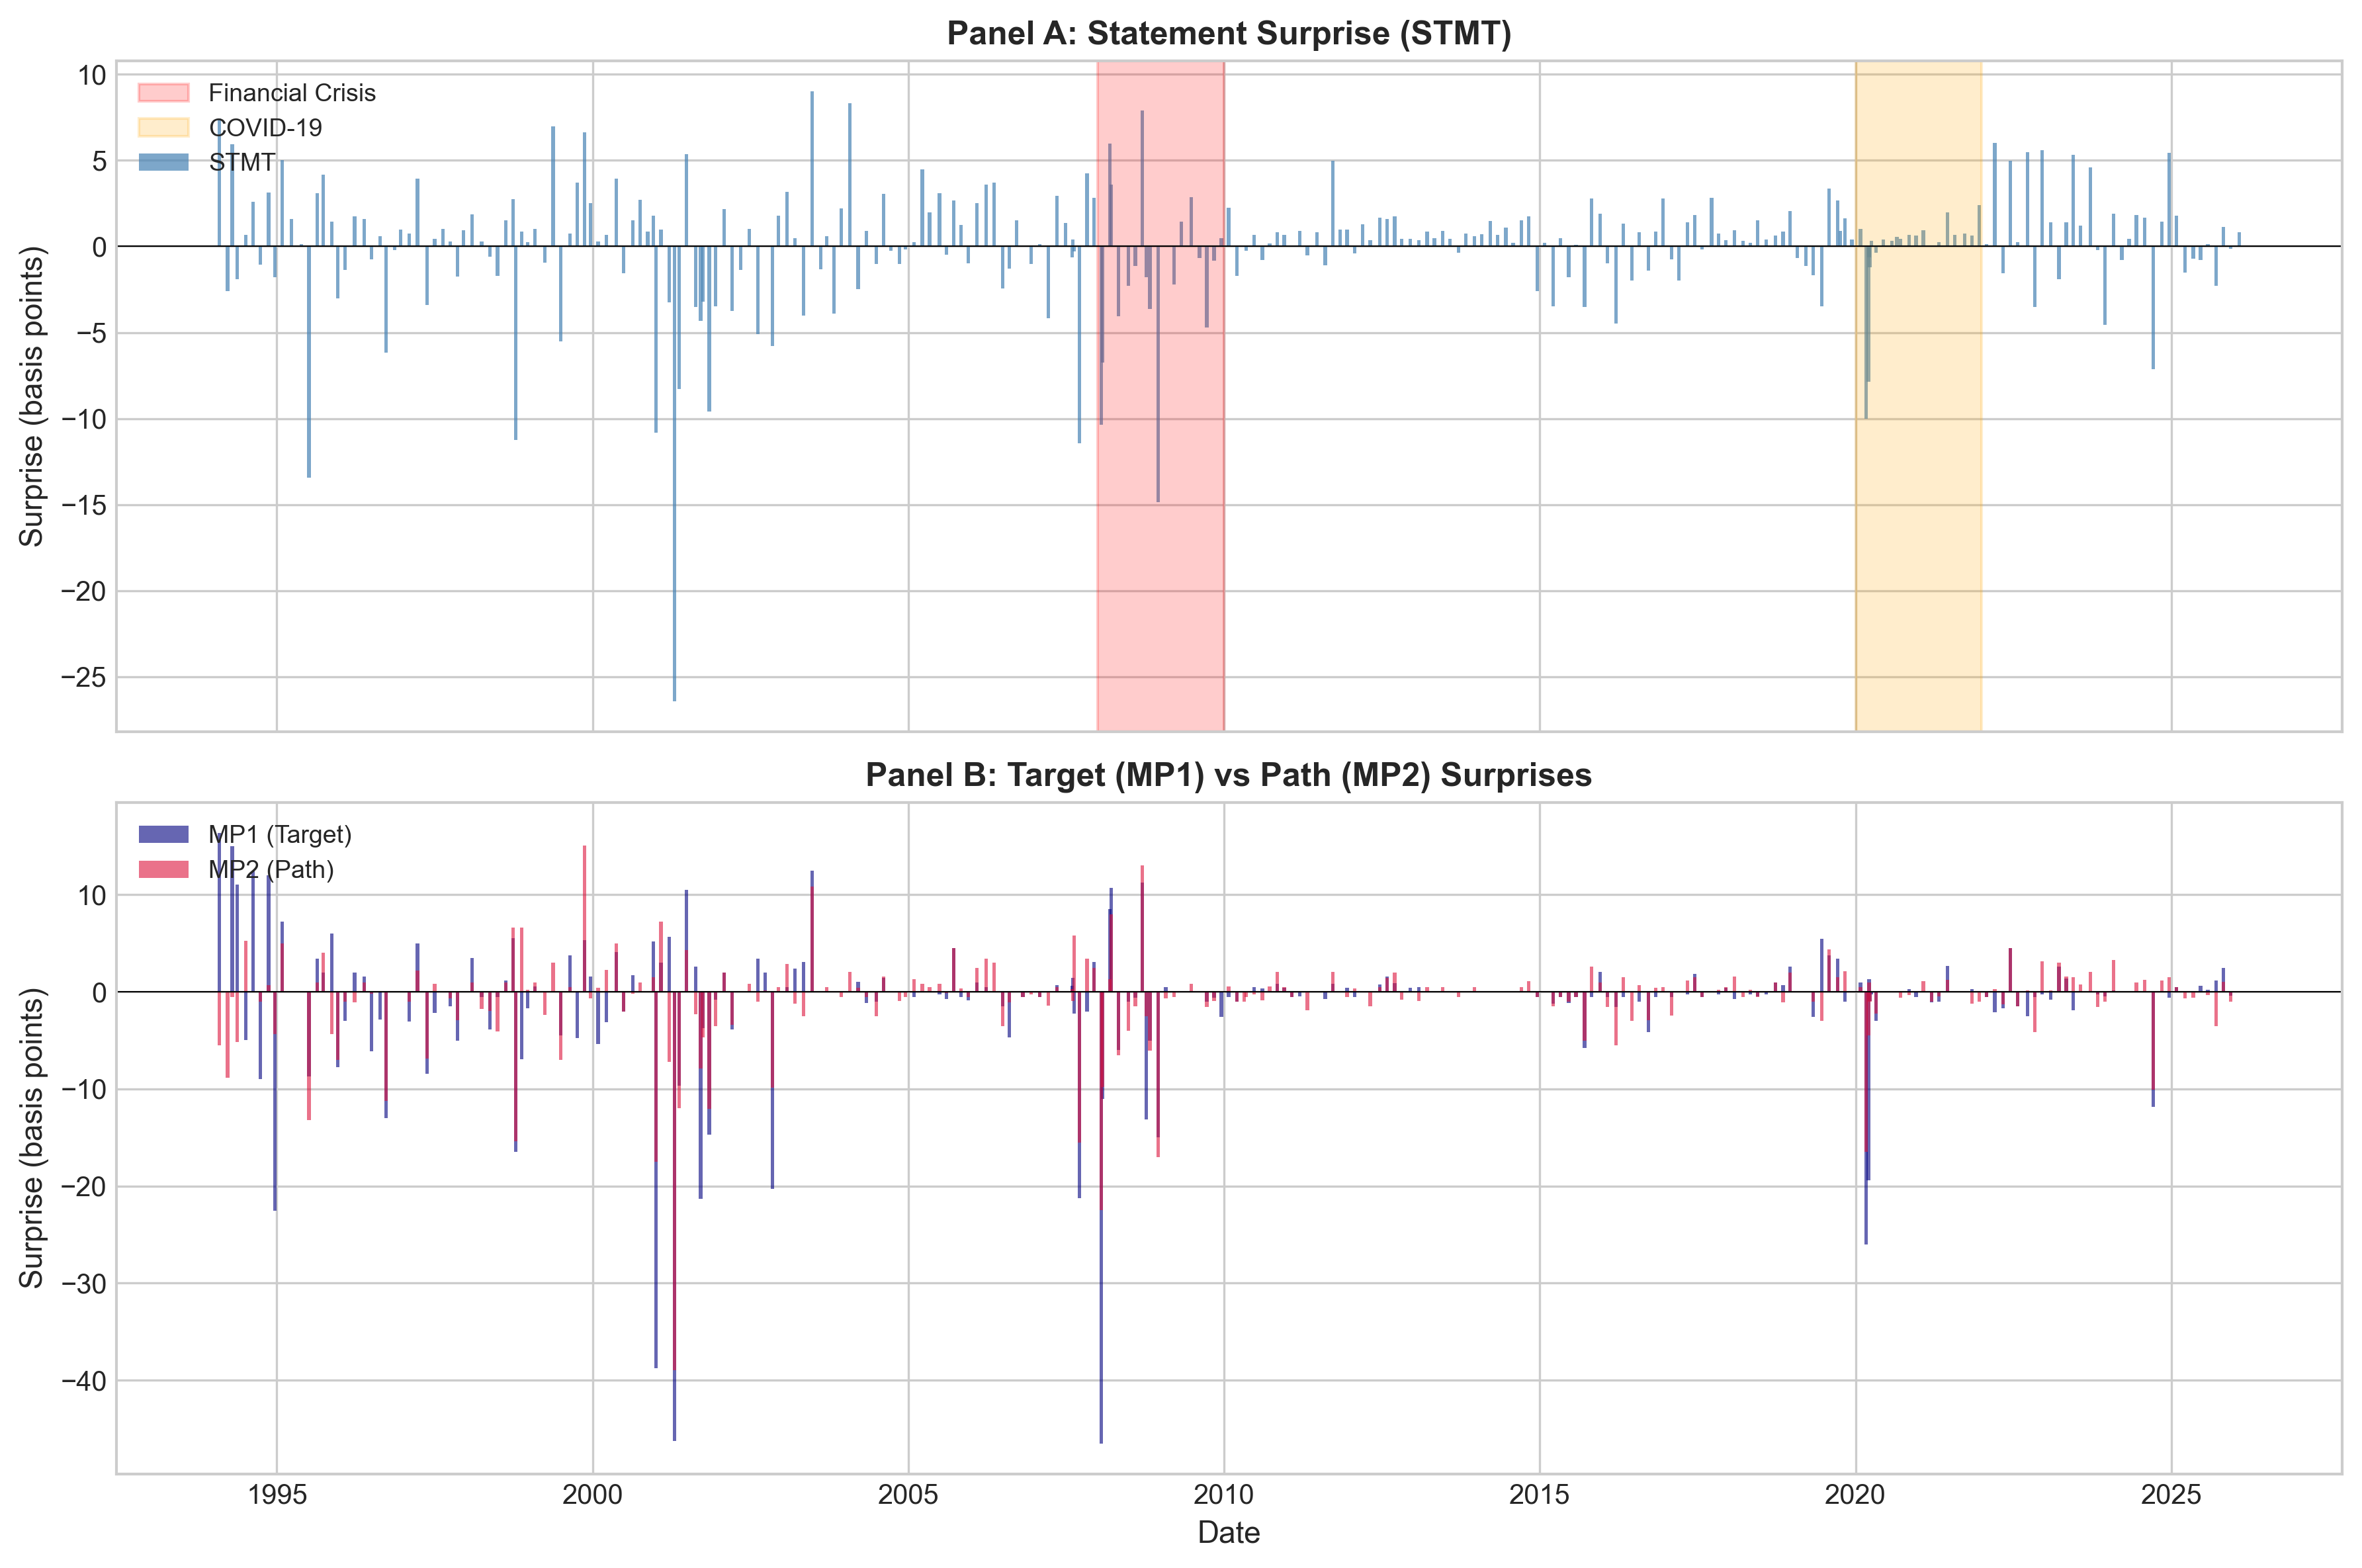
\includegraphics[width=\textwidth]{figure1_surprise_timeseries.png}
\caption{Monetary policy surprise time series (STMT, MP1, MP2), 1994--2024.}
\end{figure}

\clearpage
% ----------------------------------------------------------------------------
\section{Figure 2: Correlation Heatmap}
\begin{figure}[H]
\centering
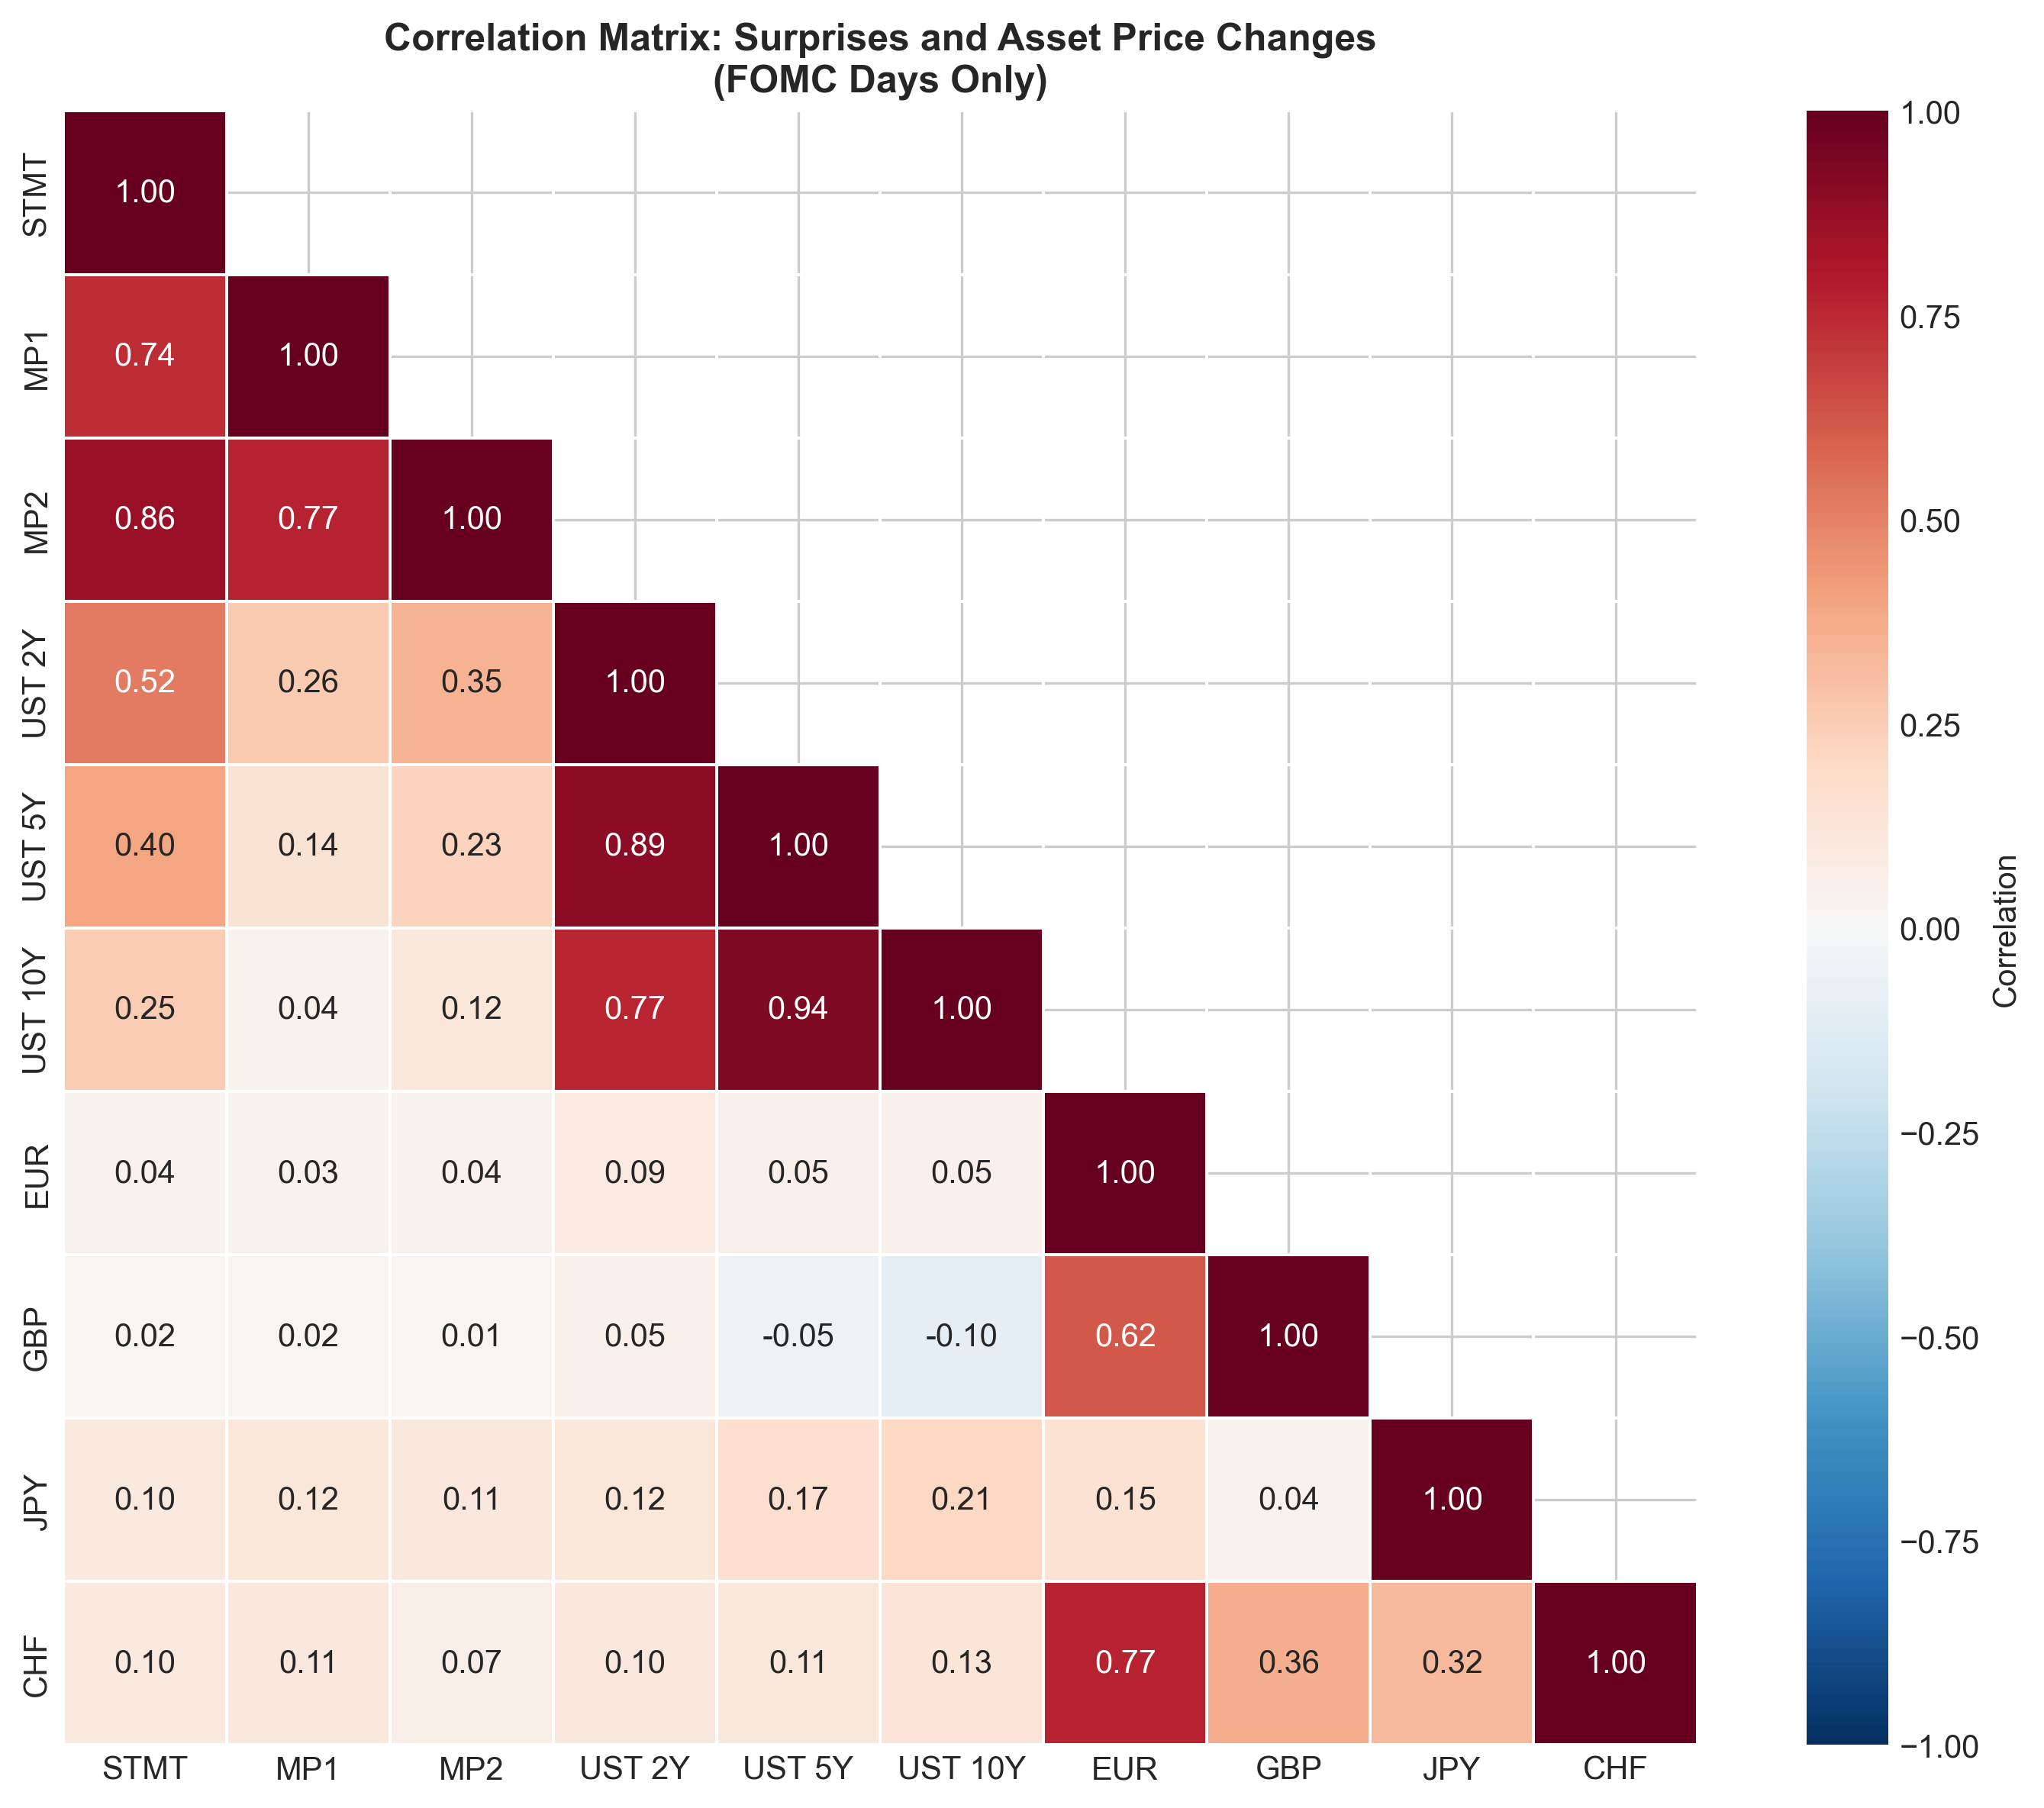
\includegraphics[width=\textwidth]{figure2_correlation_heatmap.png}
\caption{Correlation heatmap of monetary policy surprises and asset price changes.}
\end{figure}

\clearpage
% ----------------------------------------------------------------------------
\section{Figure 3: Surprise Distributions}
\begin{figure}[H]
\centering
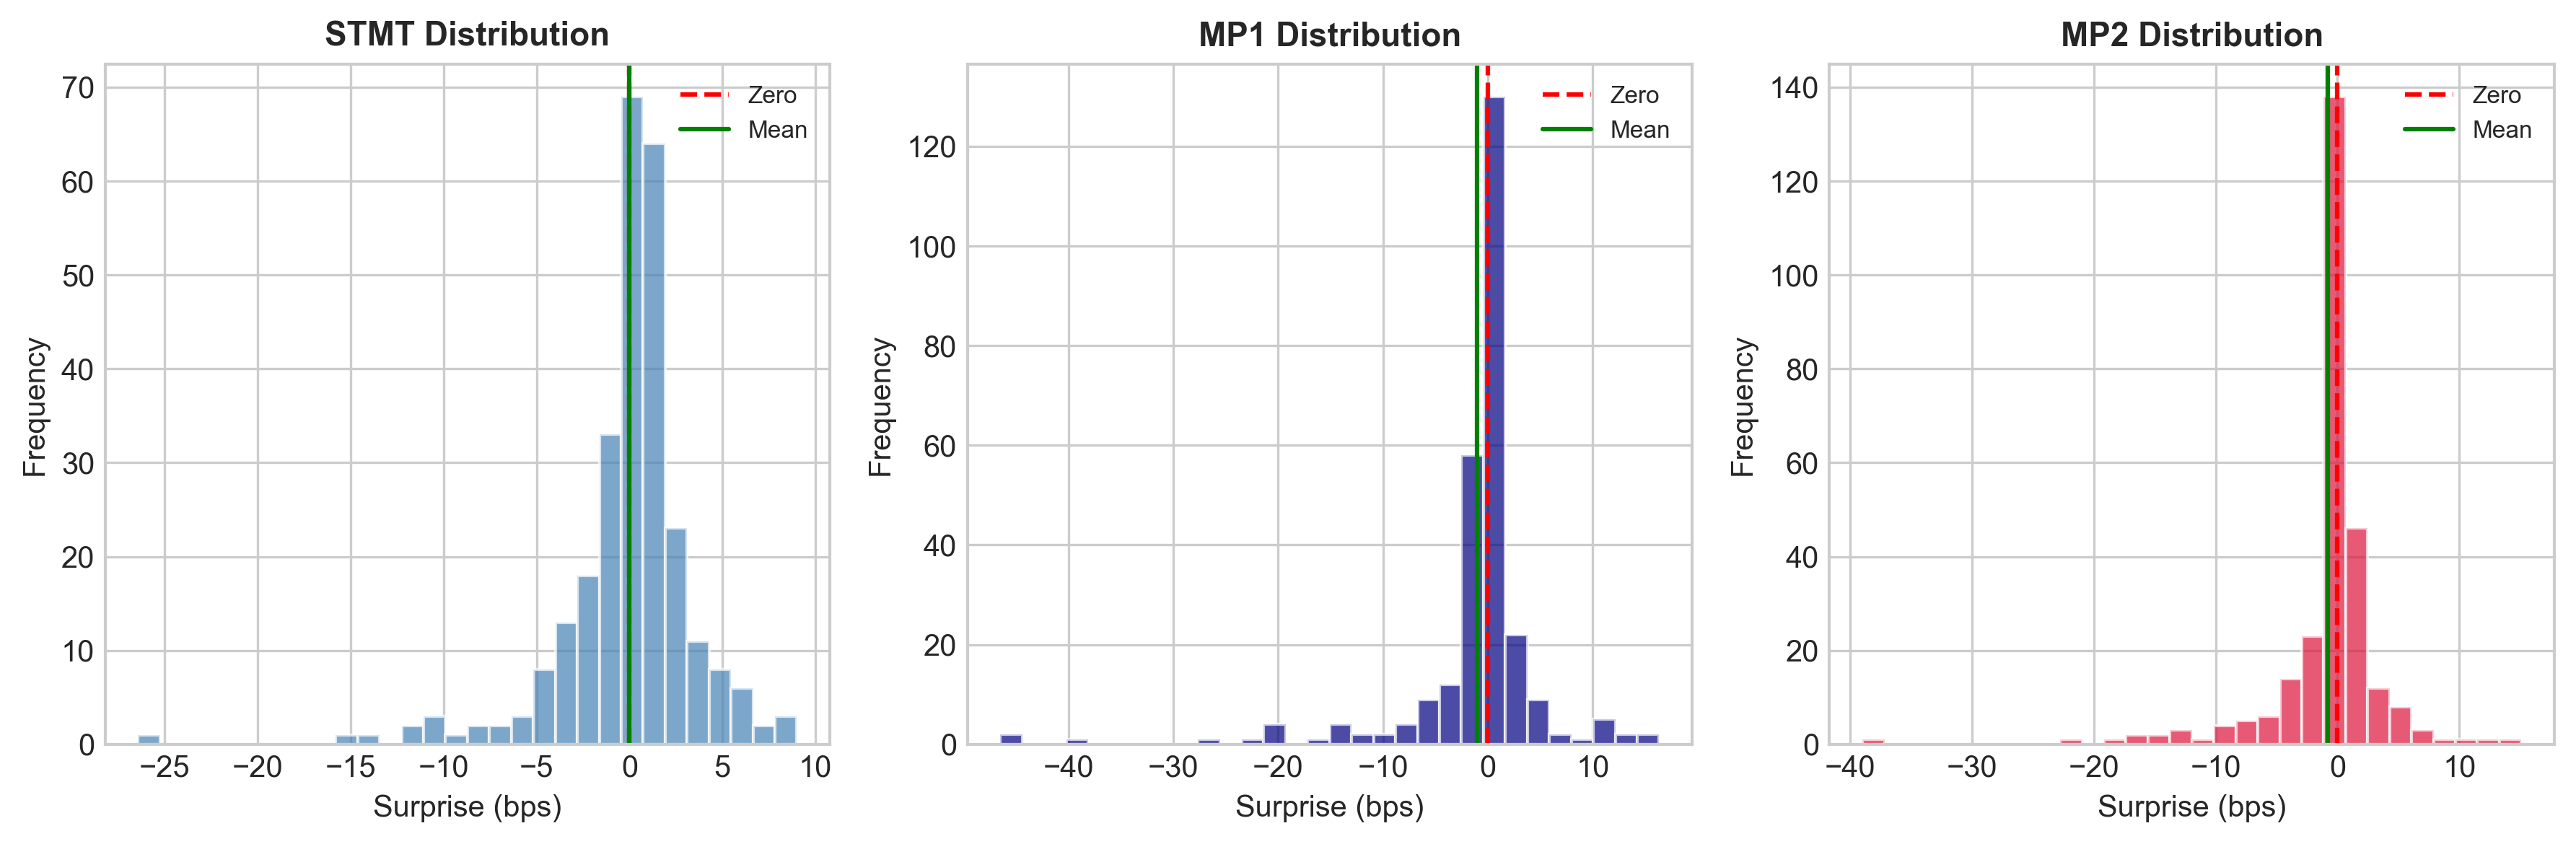
\includegraphics[width=\textwidth]{figure3_surprise_distributions.png}
\caption{Distribution of monetary policy surprise measures.}
\end{figure}

\clearpage
% ----------------------------------------------------------------------------
\section{Figure 4: STMT Validation}
\begin{figure}[H]
\centering
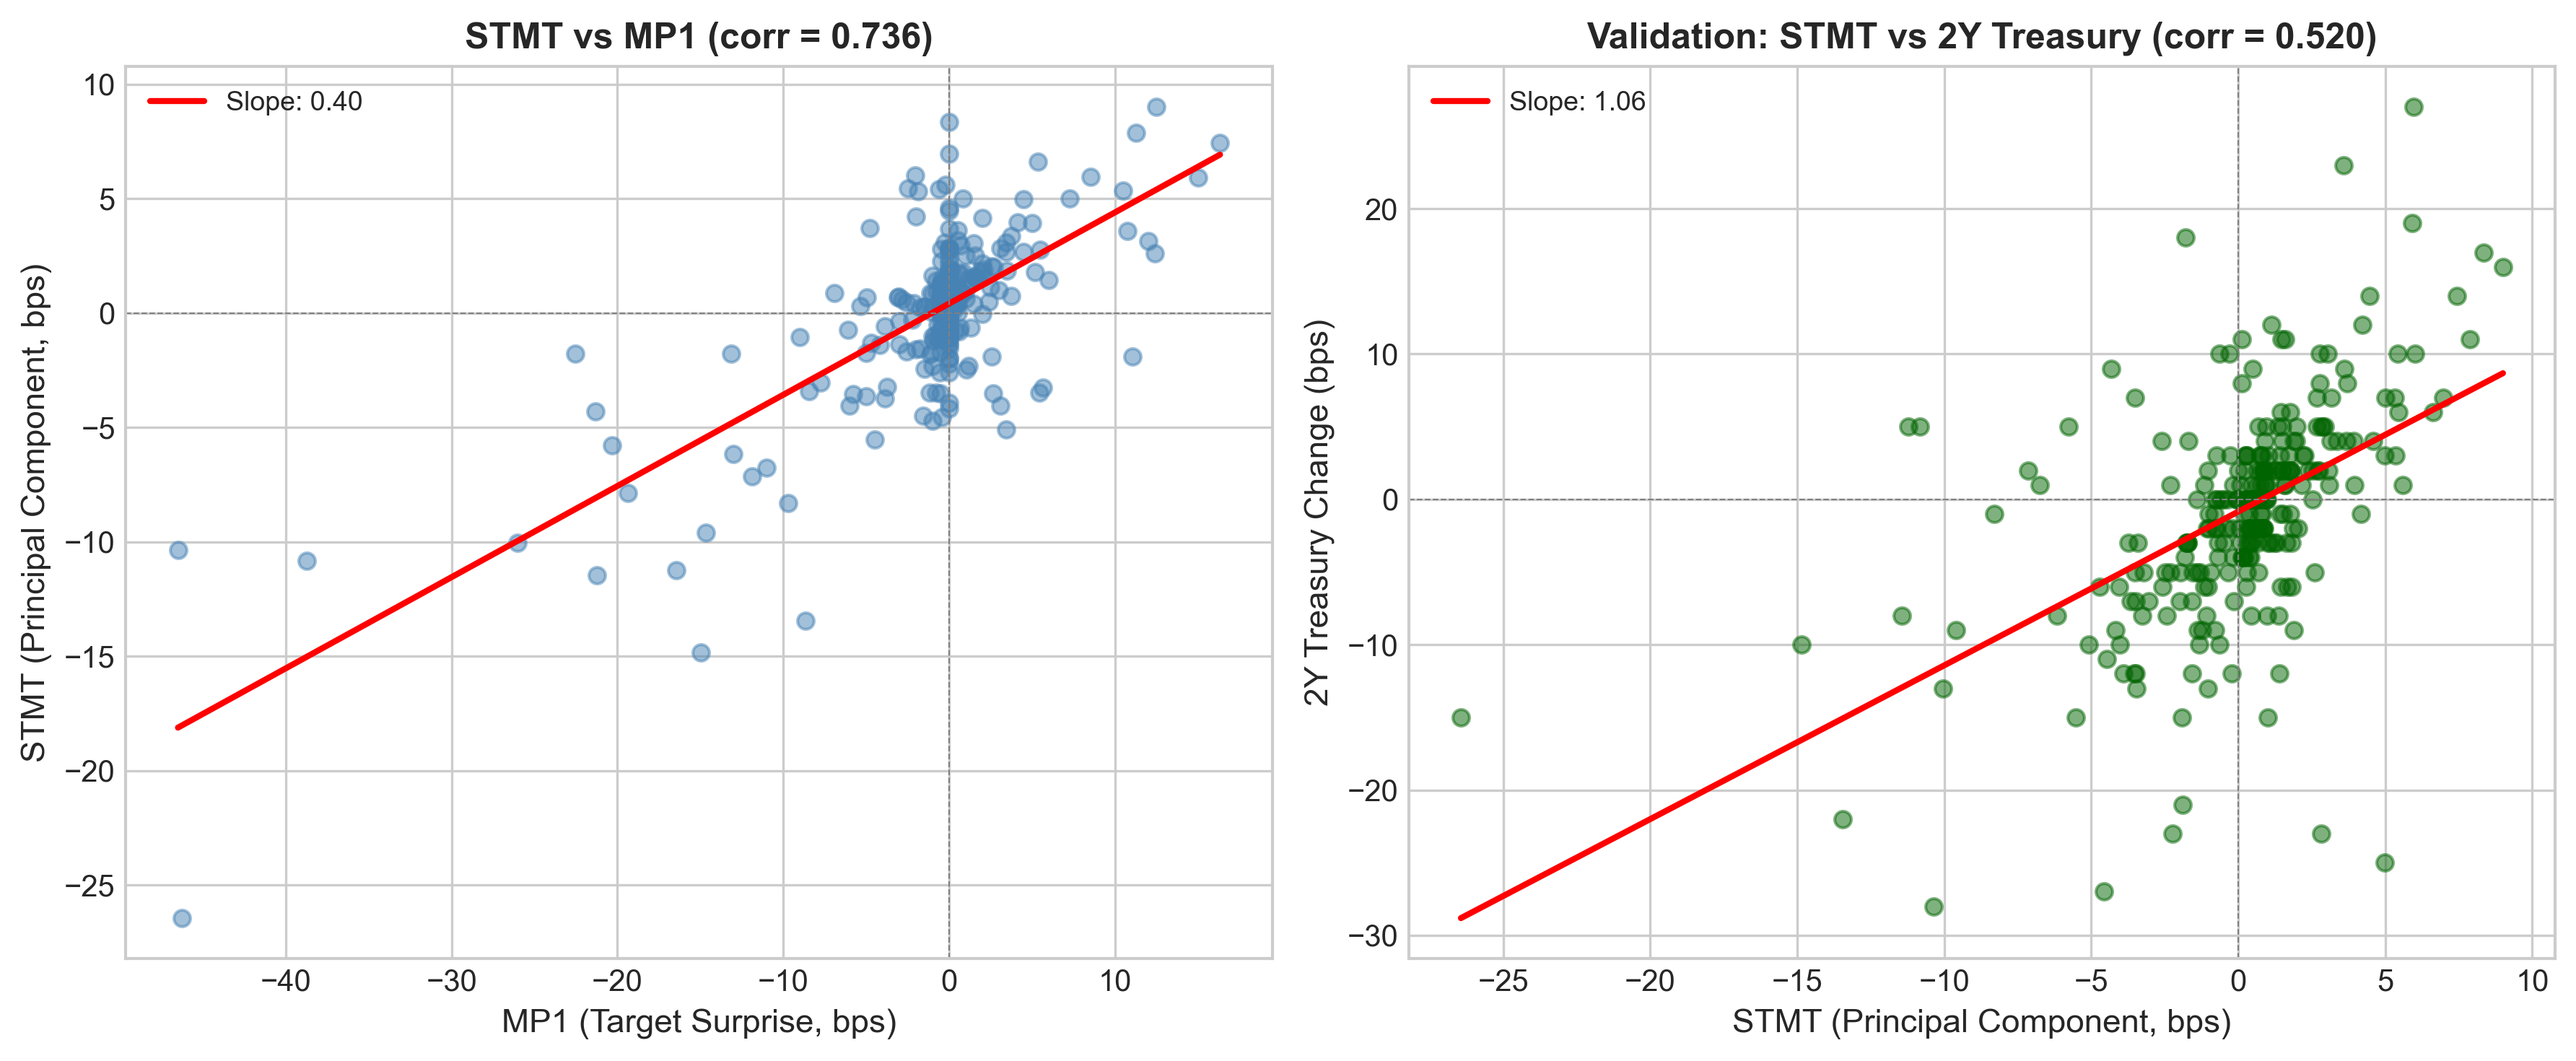
\includegraphics[width=\textwidth]{figure4_stmt_validation.png}
\caption{STMT validation: 2-year Treasury response to monetary policy surprises.}
\end{figure}

\clearpage
% ----------------------------------------------------------------------------
\section{Figure 5: Event Scatter}
\begin{figure}[H]
\centering
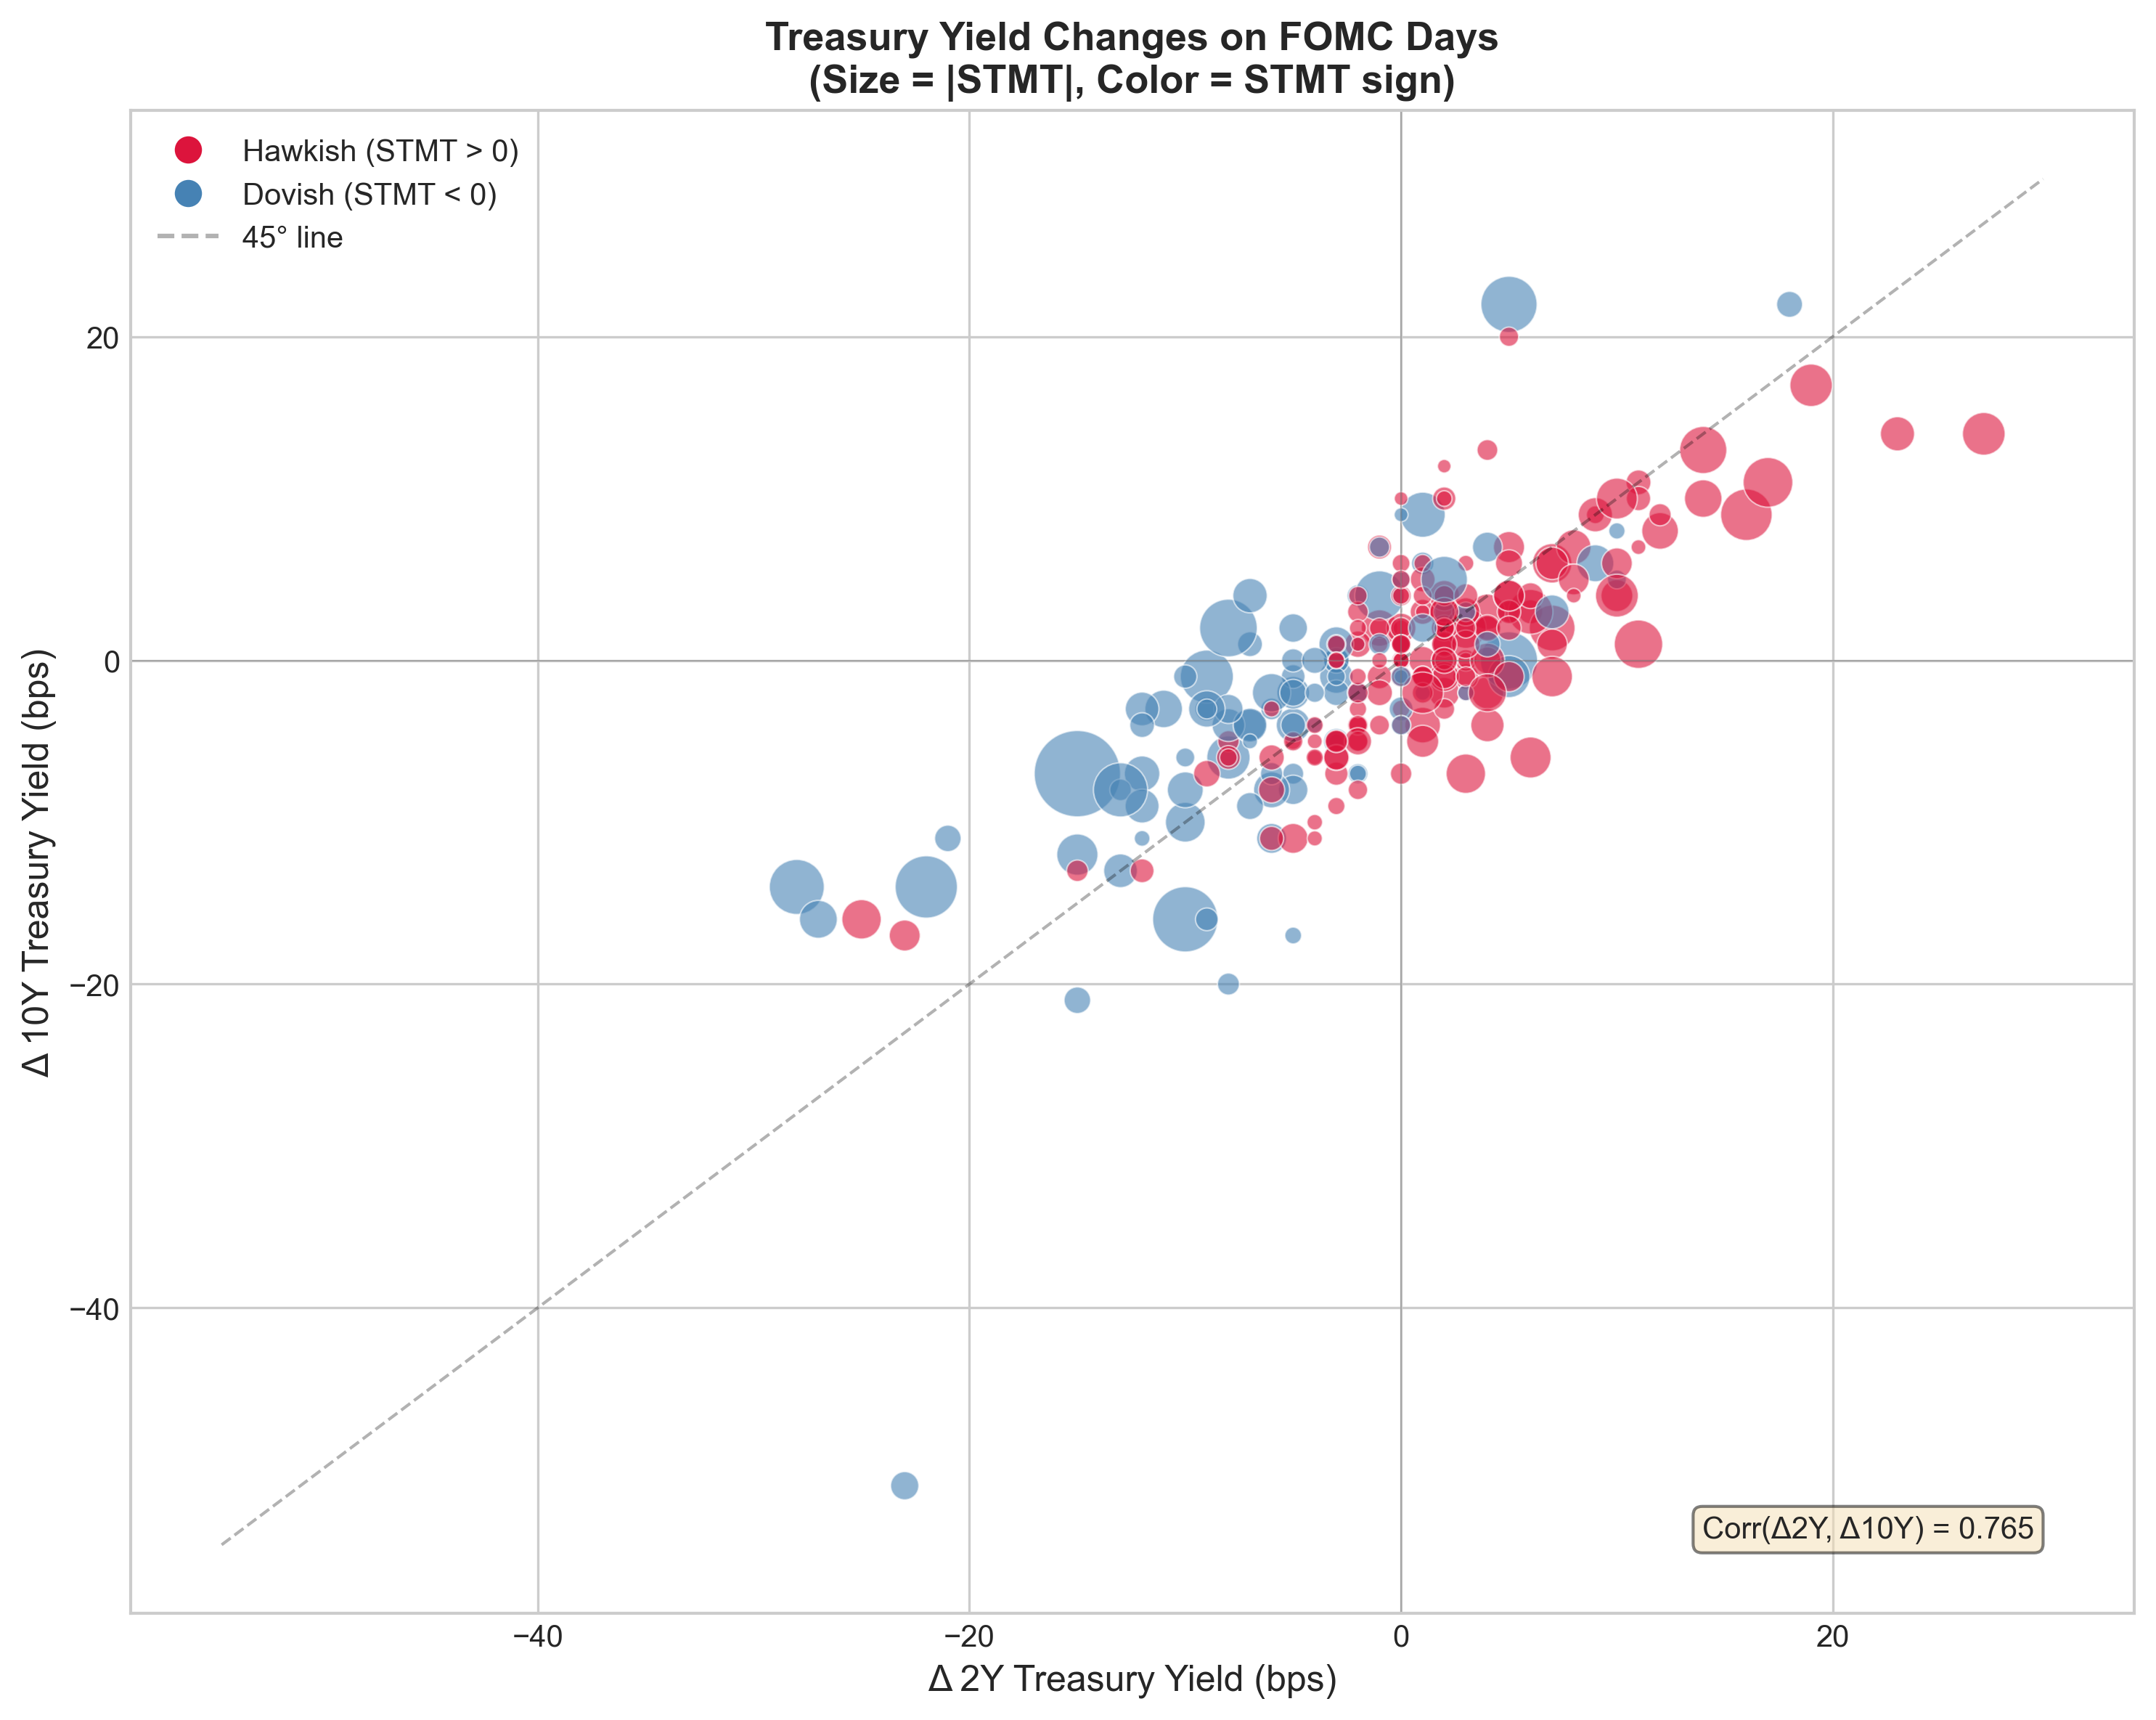
\includegraphics[width=\textwidth]{figure5_event_scatter.png}
\caption{Scatter plot of FX changes vs.\ monetary policy surprises on FOMC dates.}
\end{figure}

\clearpage
% ----------------------------------------------------------------------------
\section{Figure 6: Volatility by Period}
\begin{figure}[H]
\centering
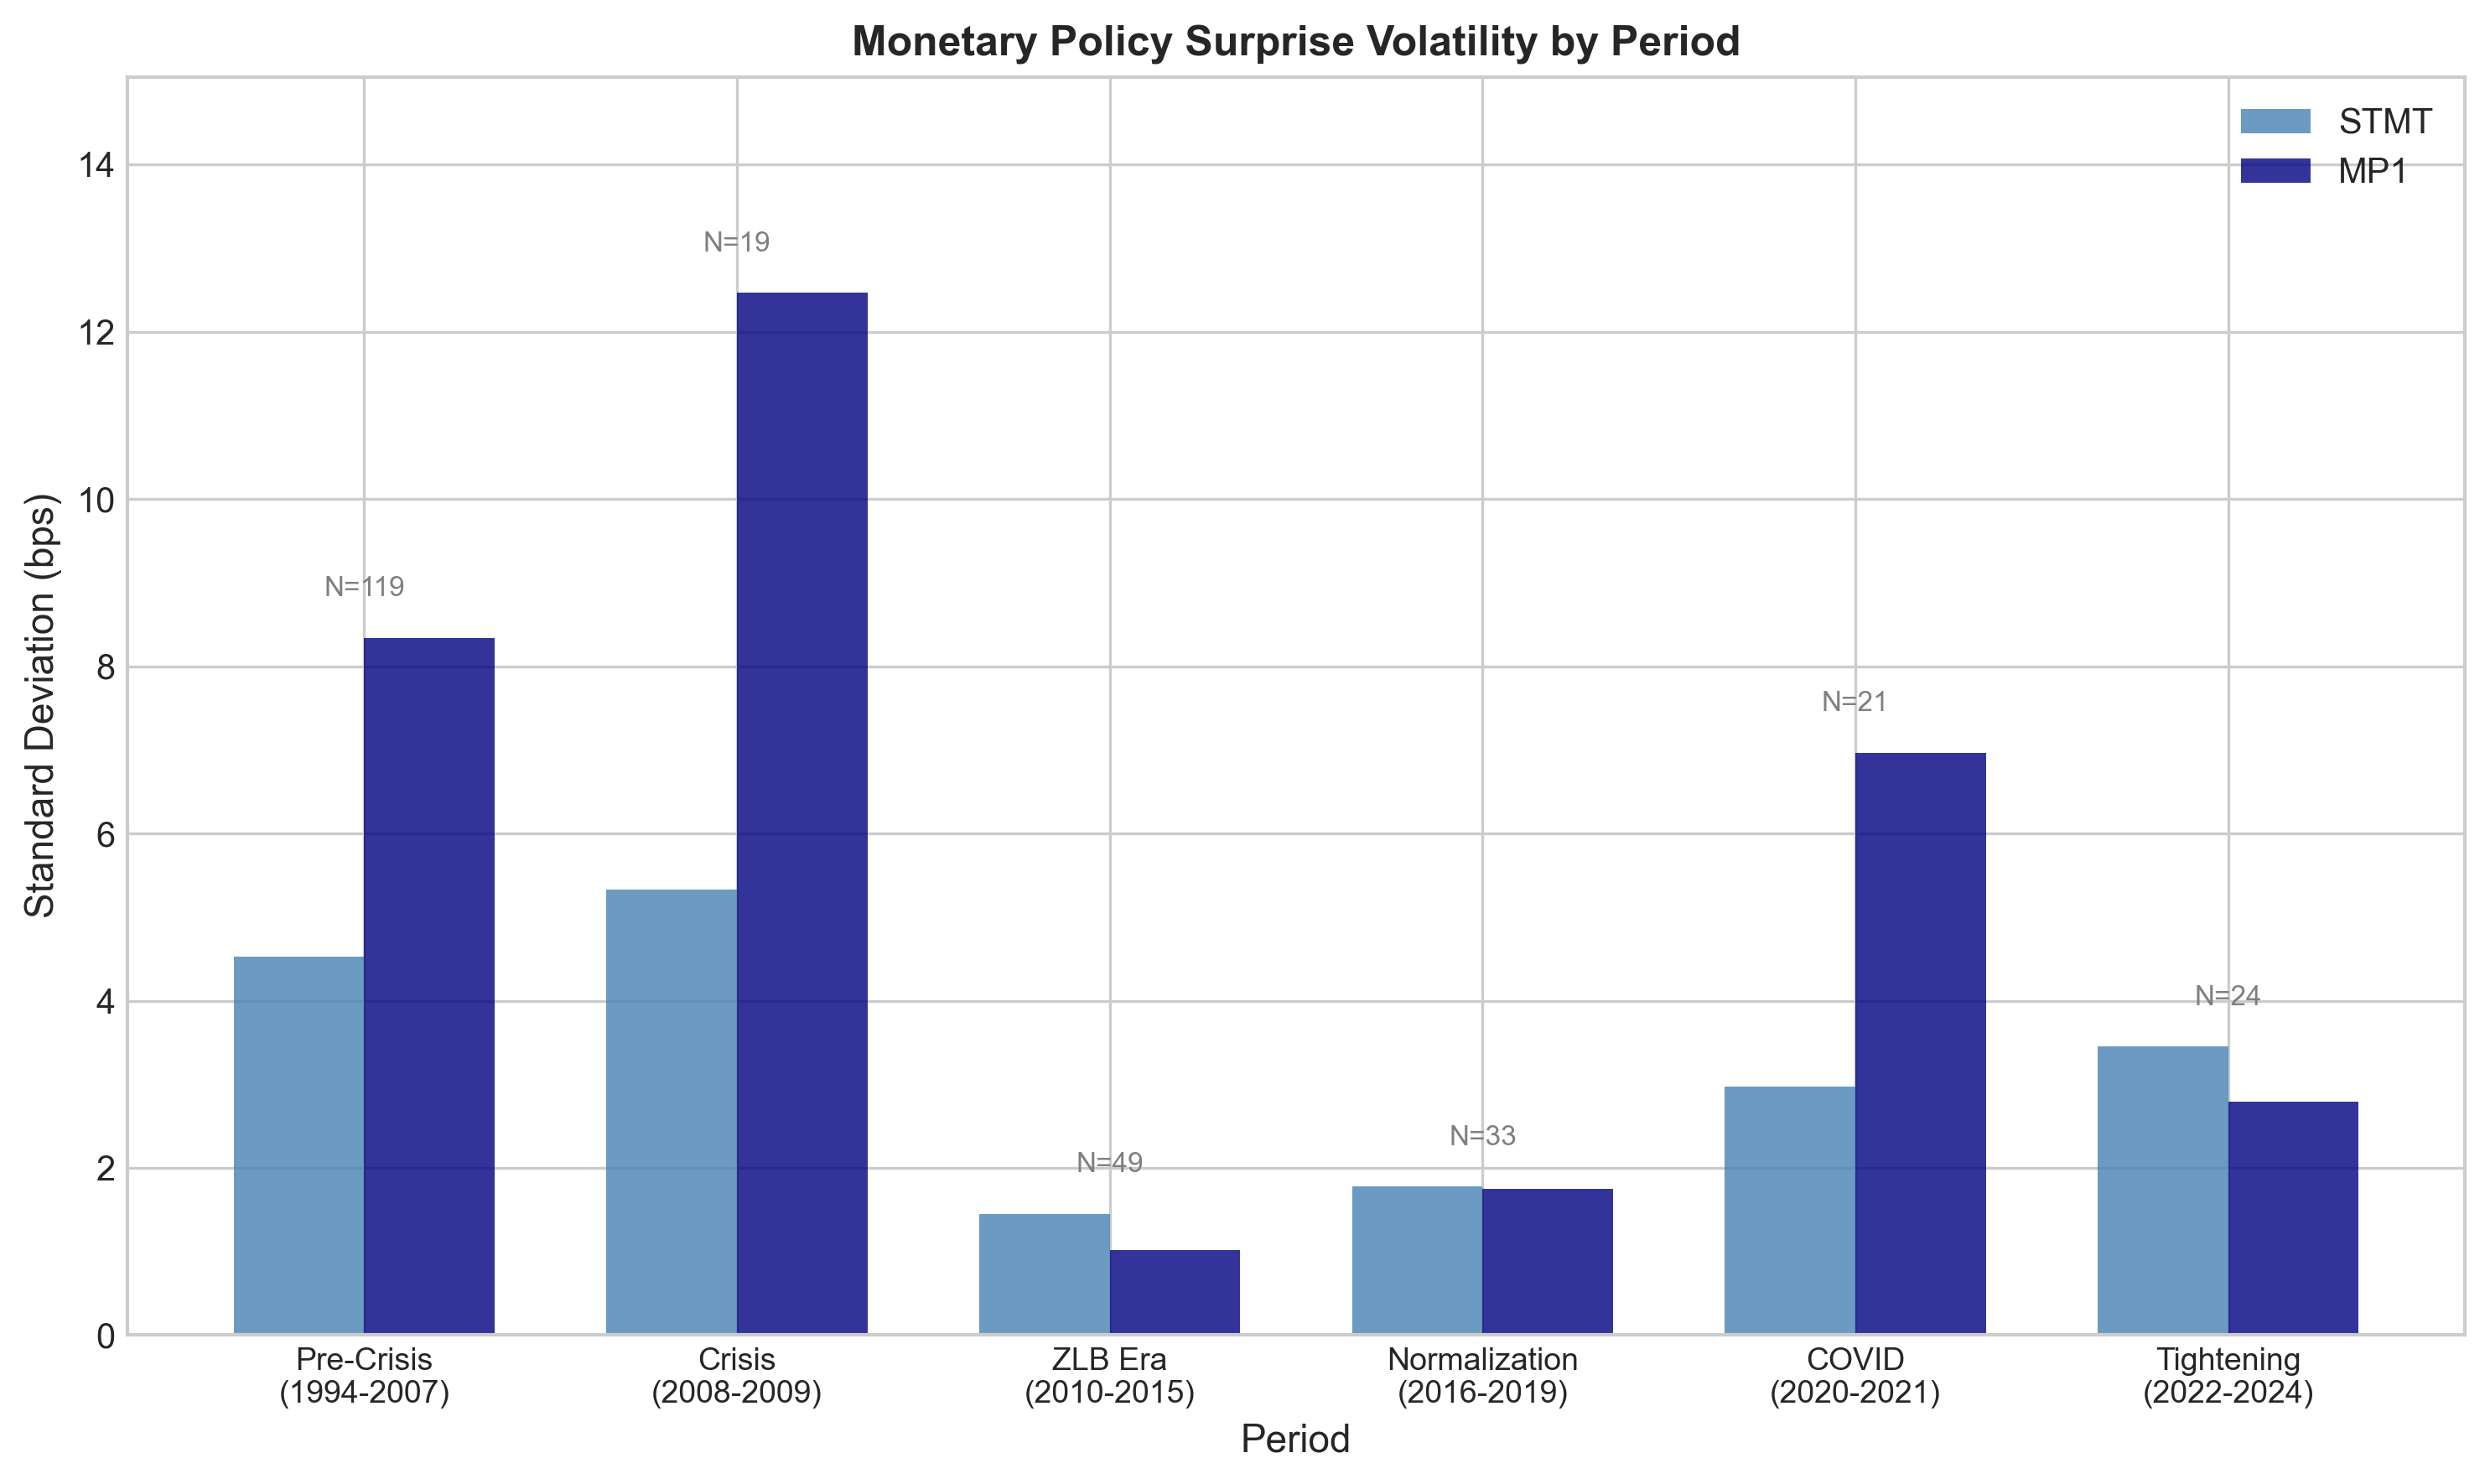
\includegraphics[width=\textwidth]{figure6_volatility_by_period.png}
\caption{FX volatility by sub-period (pre-GFC, GFC, post-GFC).}
\end{figure}

\clearpage
% ----------------------------------------------------------------------------
\section{Figure 7: Term Structure Response}
\begin{figure}[H]
\centering
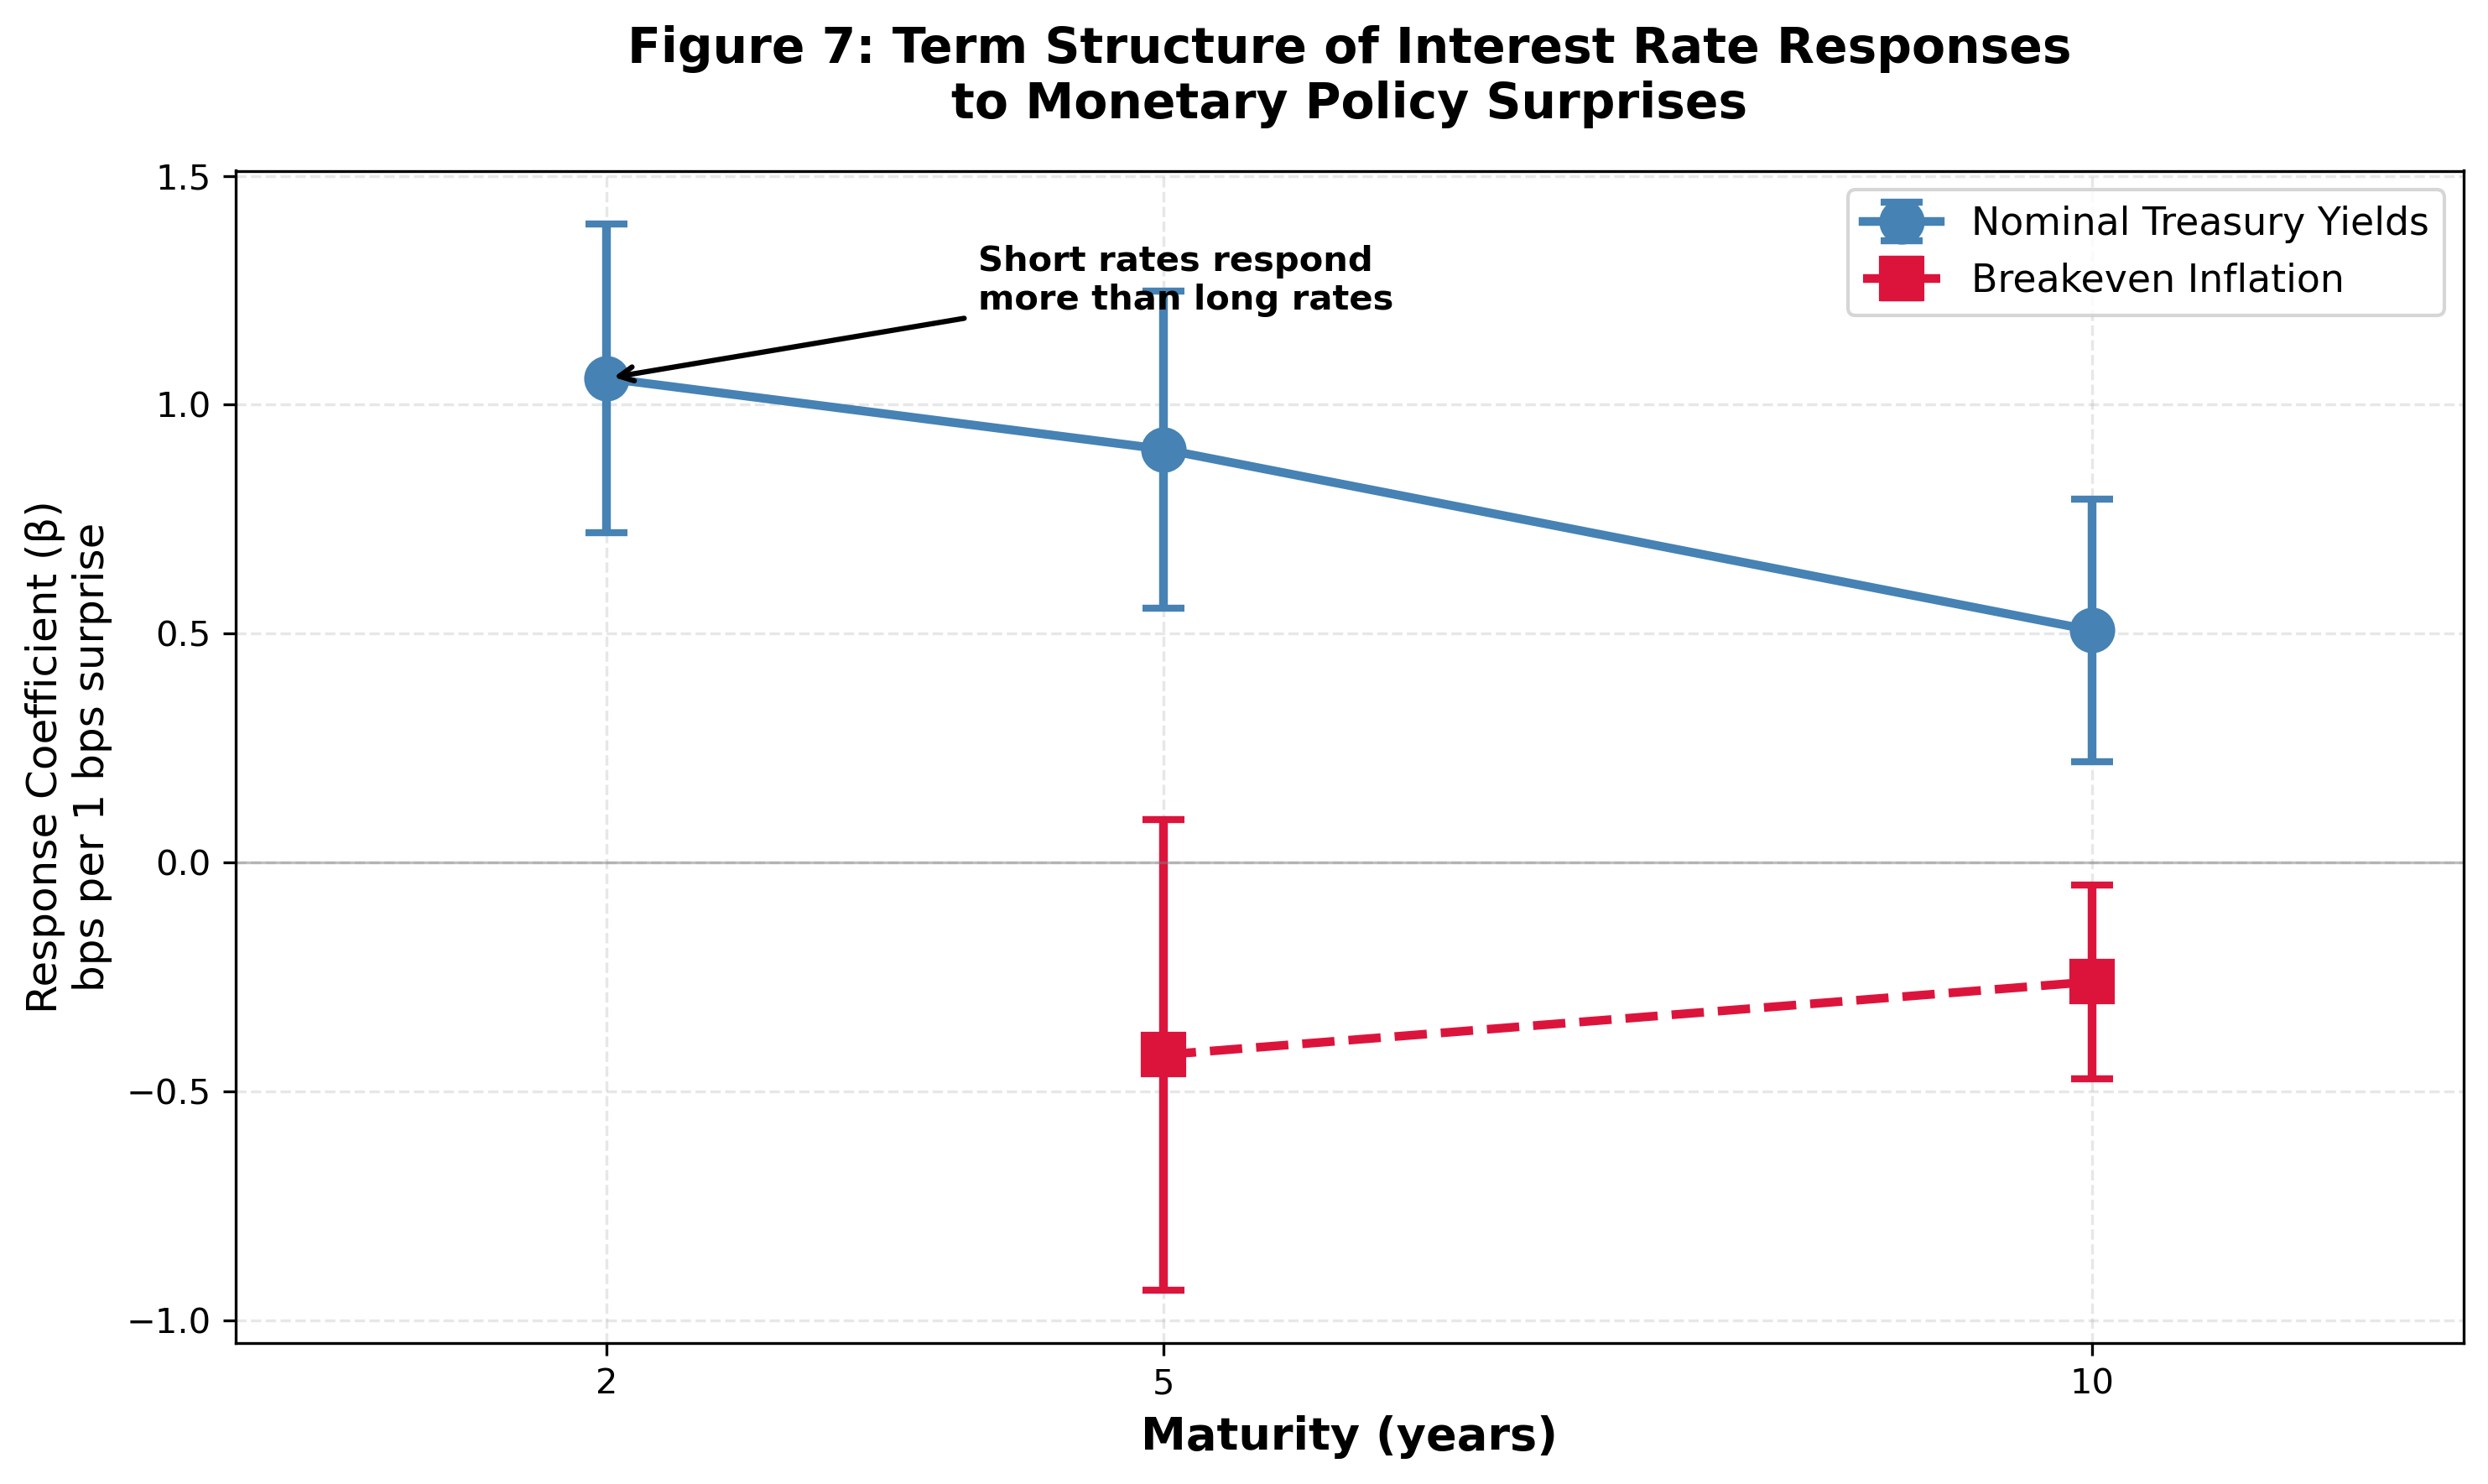
\includegraphics[width=\textwidth]{figure7_term_structure.png}
\caption{Treasury yield response across the term structure.}
\end{figure}

\clearpage
% ----------------------------------------------------------------------------
\section{Figure 8: FX Heterogeneity}
\begin{figure}[H]
\centering
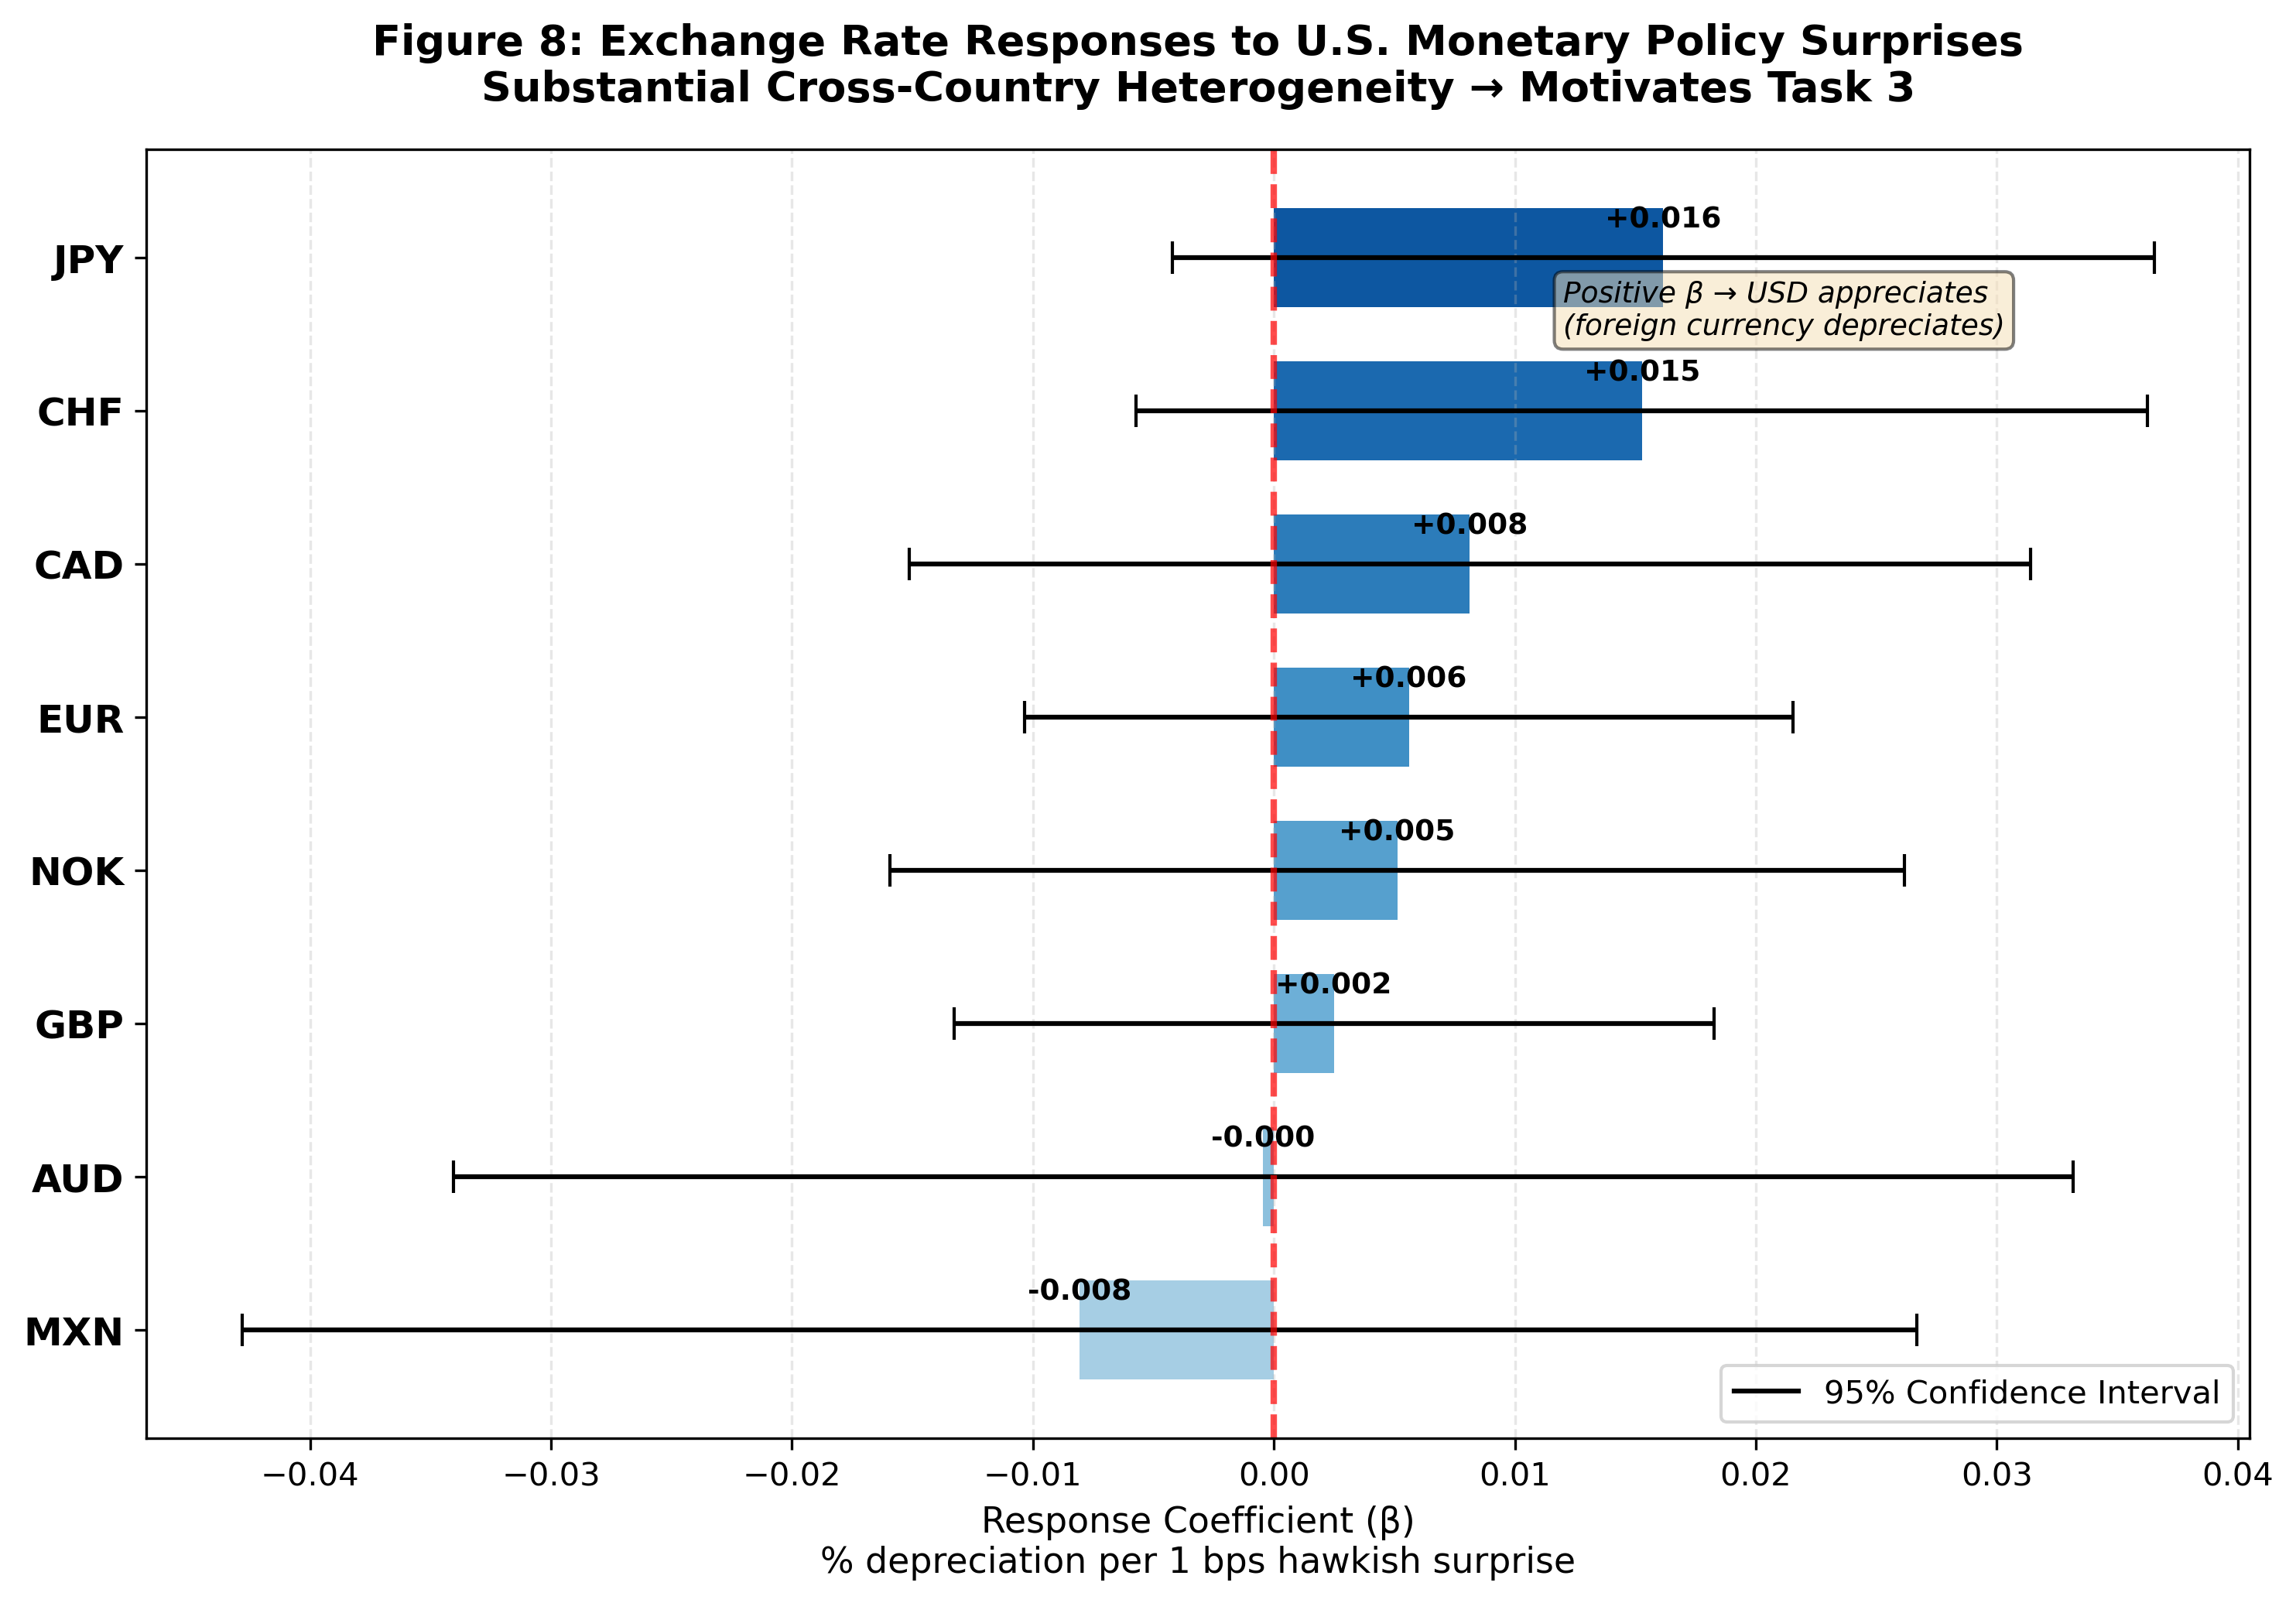
\includegraphics[width=\textwidth]{figure8_fx_heterogeneity.png}
\caption{Cross-currency heterogeneity in FX response to monetary policy surprises.}
\end{figure}

\clearpage
% ----------------------------------------------------------------------------
\section{Figure 9: Coefficient Plot}
\begin{figure}[H]
\centering
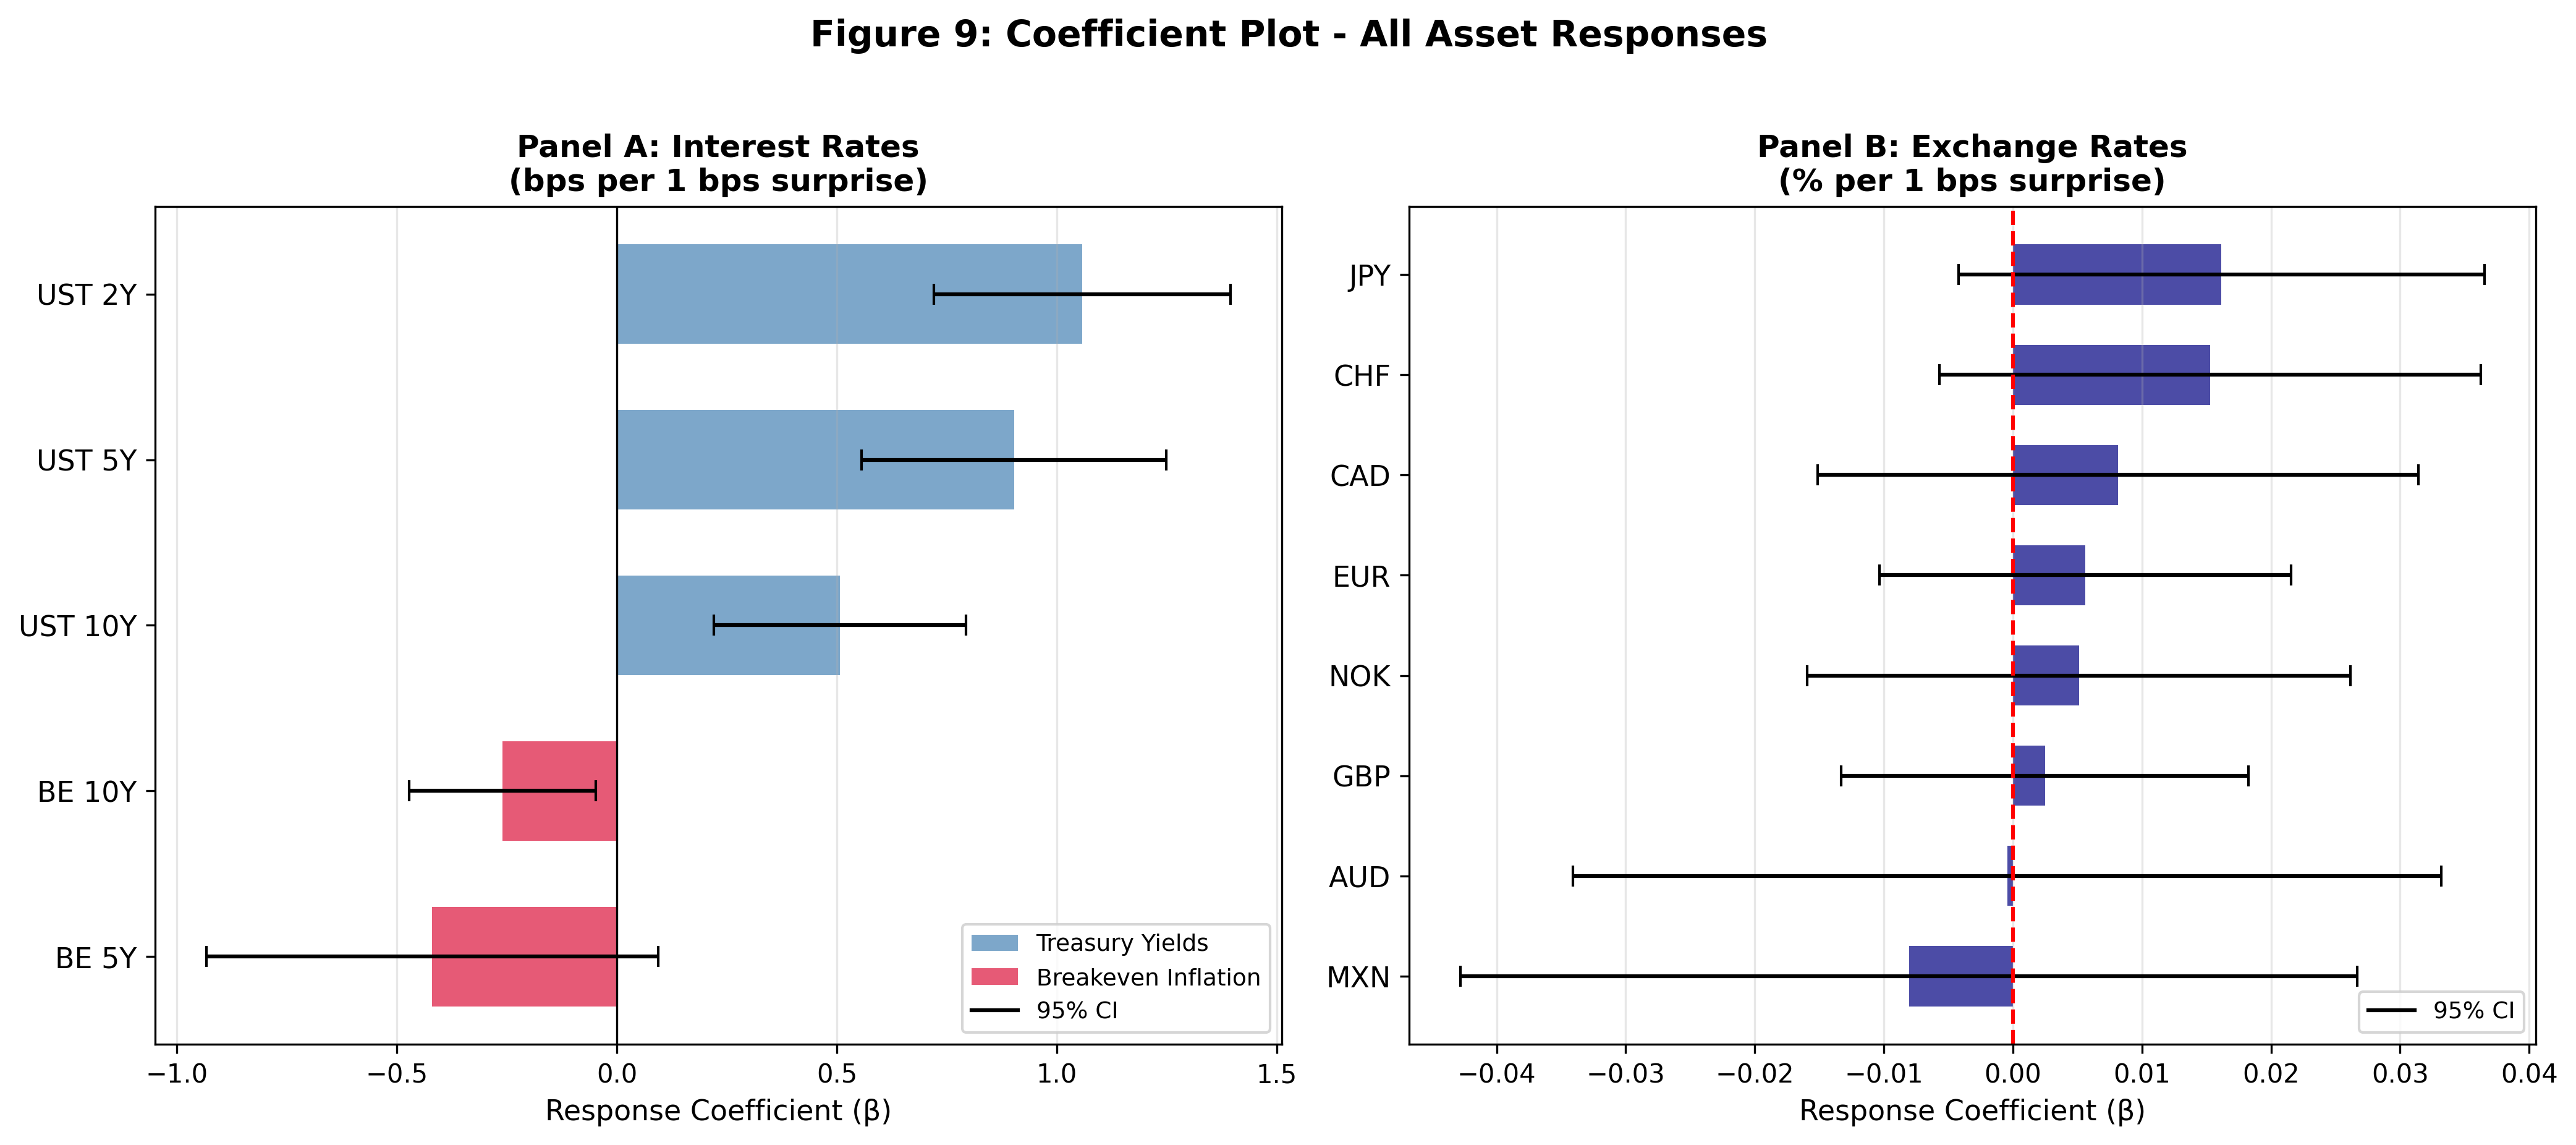
\includegraphics[width=\textwidth]{figure9_coefficient_plot.png}
\caption{Regression coefficient estimates with 95\% confidence intervals.}
\end{figure}

\clearpage
% ----------------------------------------------------------------------------
\section{Figure 10: Betas vs NFA}
\begin{figure}[H]
\centering
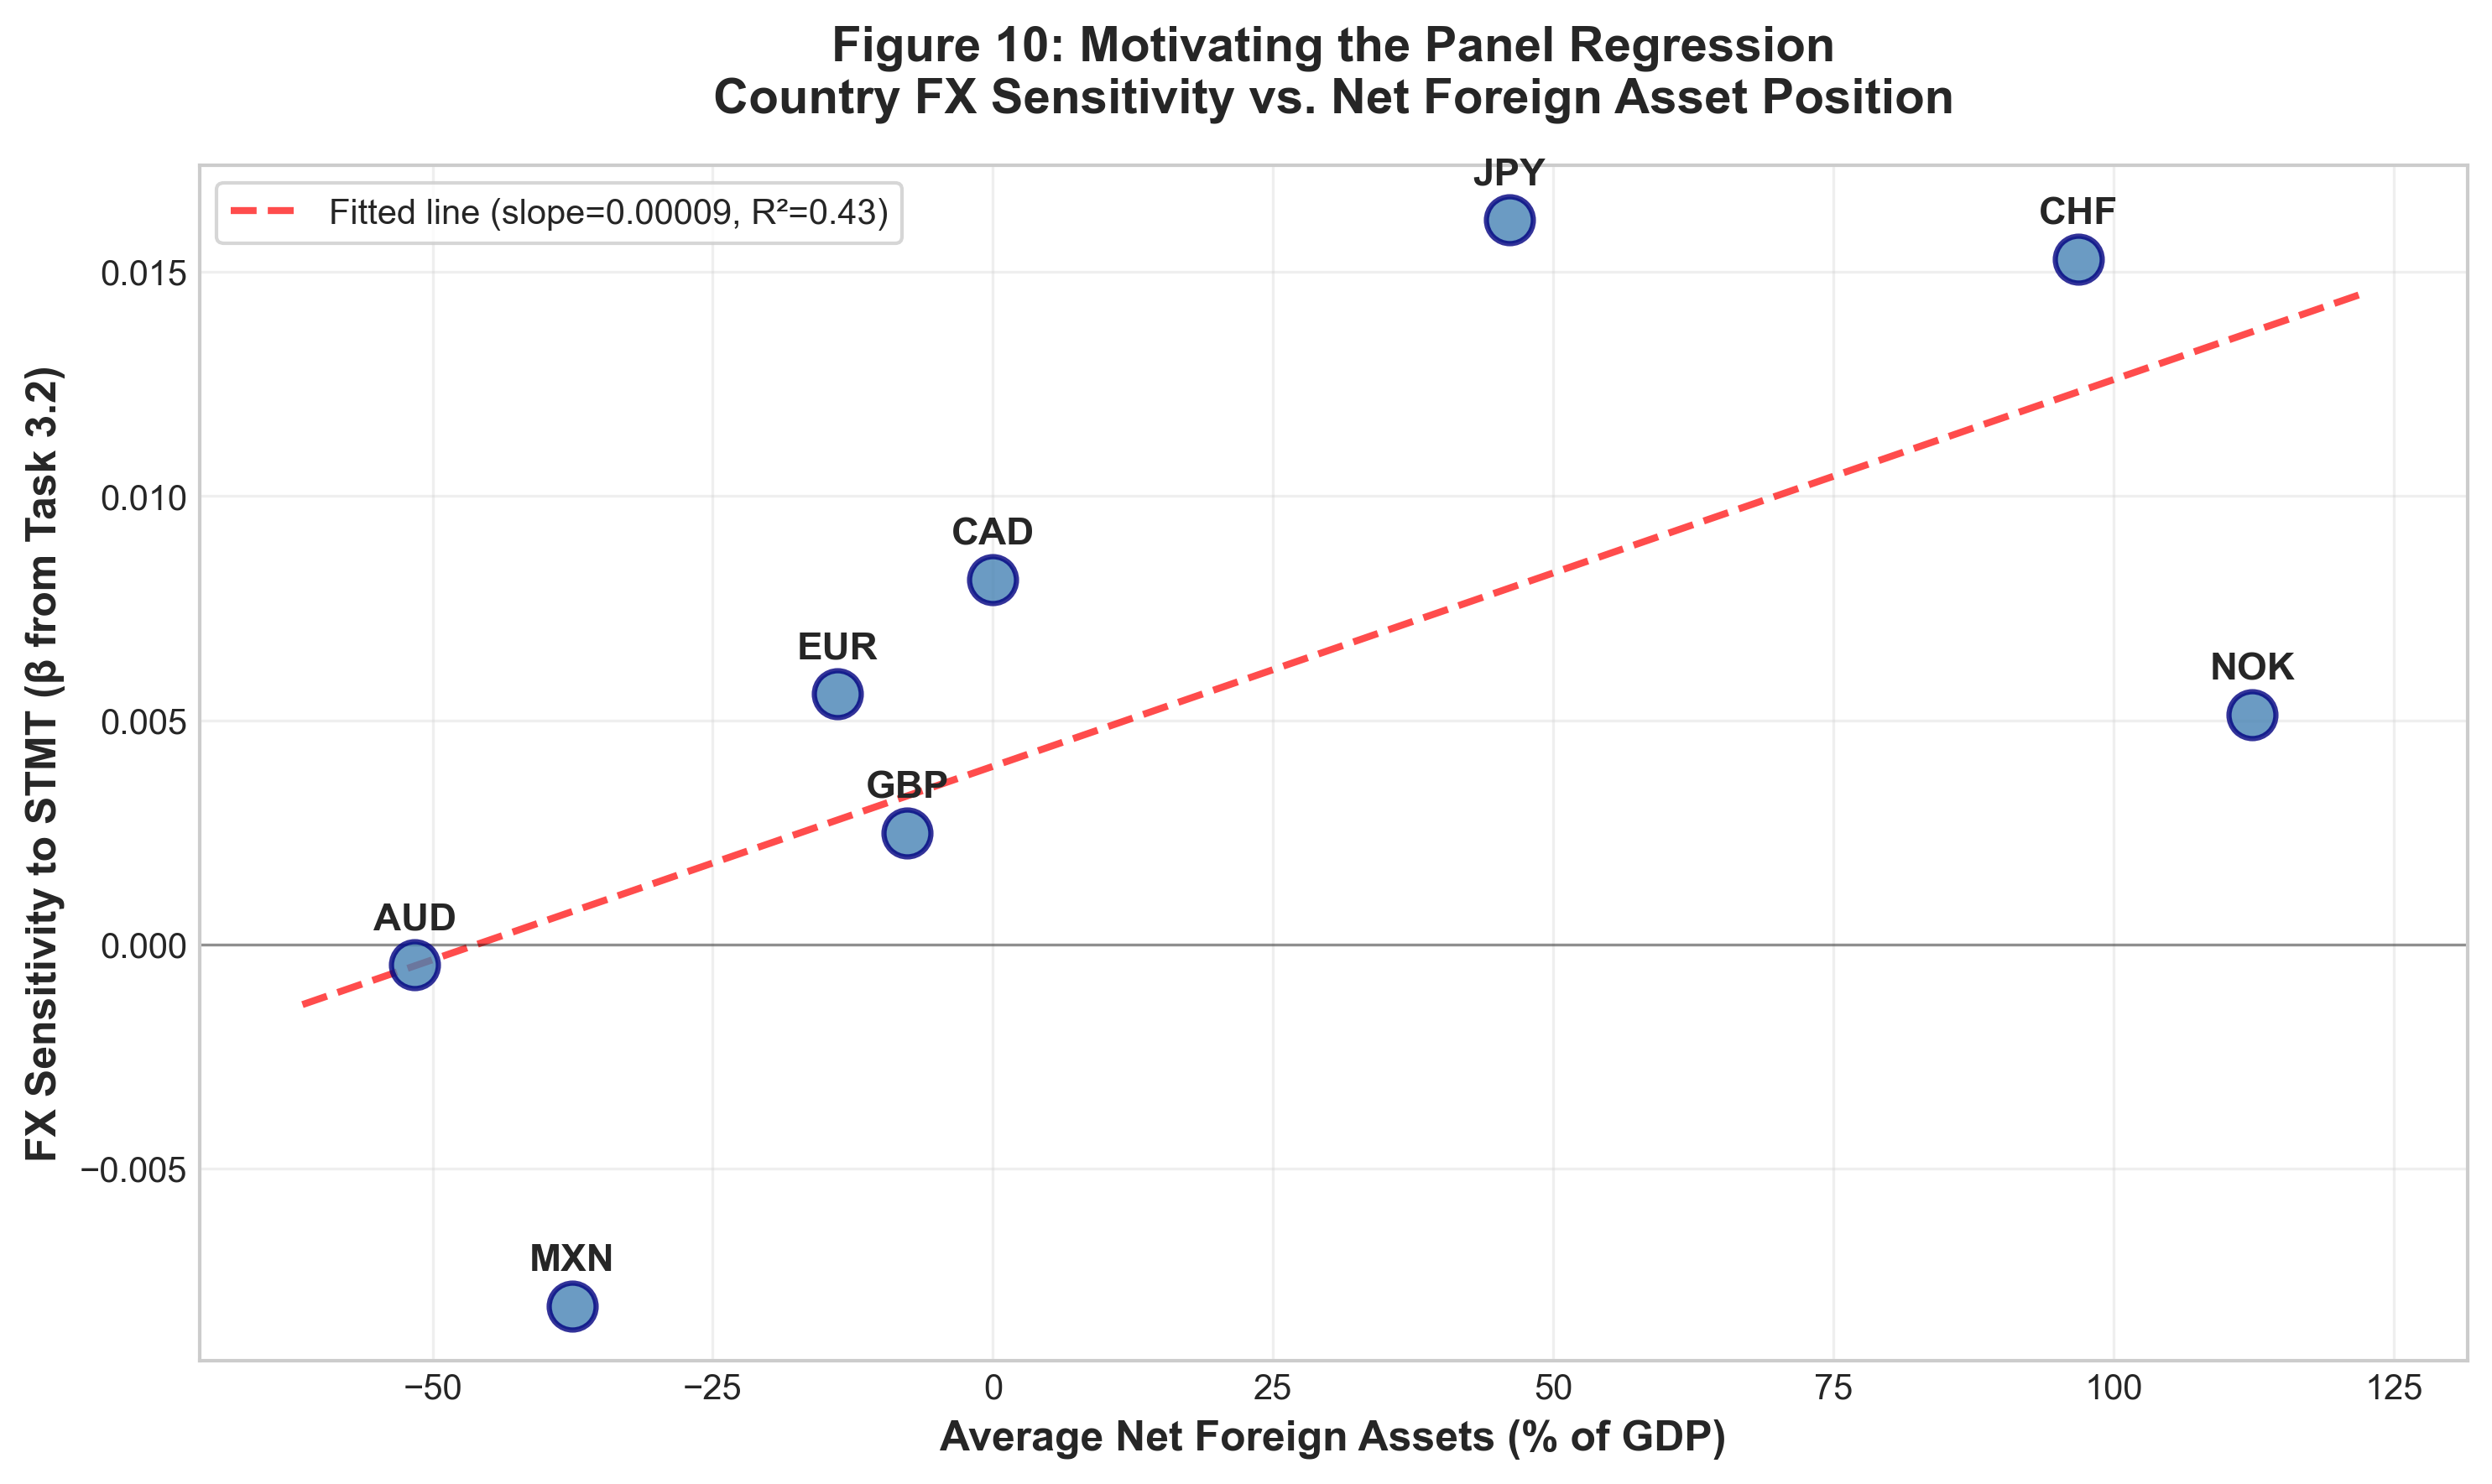
\includegraphics[width=\textwidth]{figure10_betas_vs_nfa.png}
\caption{Country-specific FX betas vs.\ NFA/GDP position.}
\end{figure}

\clearpage
% ----------------------------------------------------------------------------
\section{Figure 10b: Betas vs NFA (Both Measures)}
\begin{figure}[H]
\centering
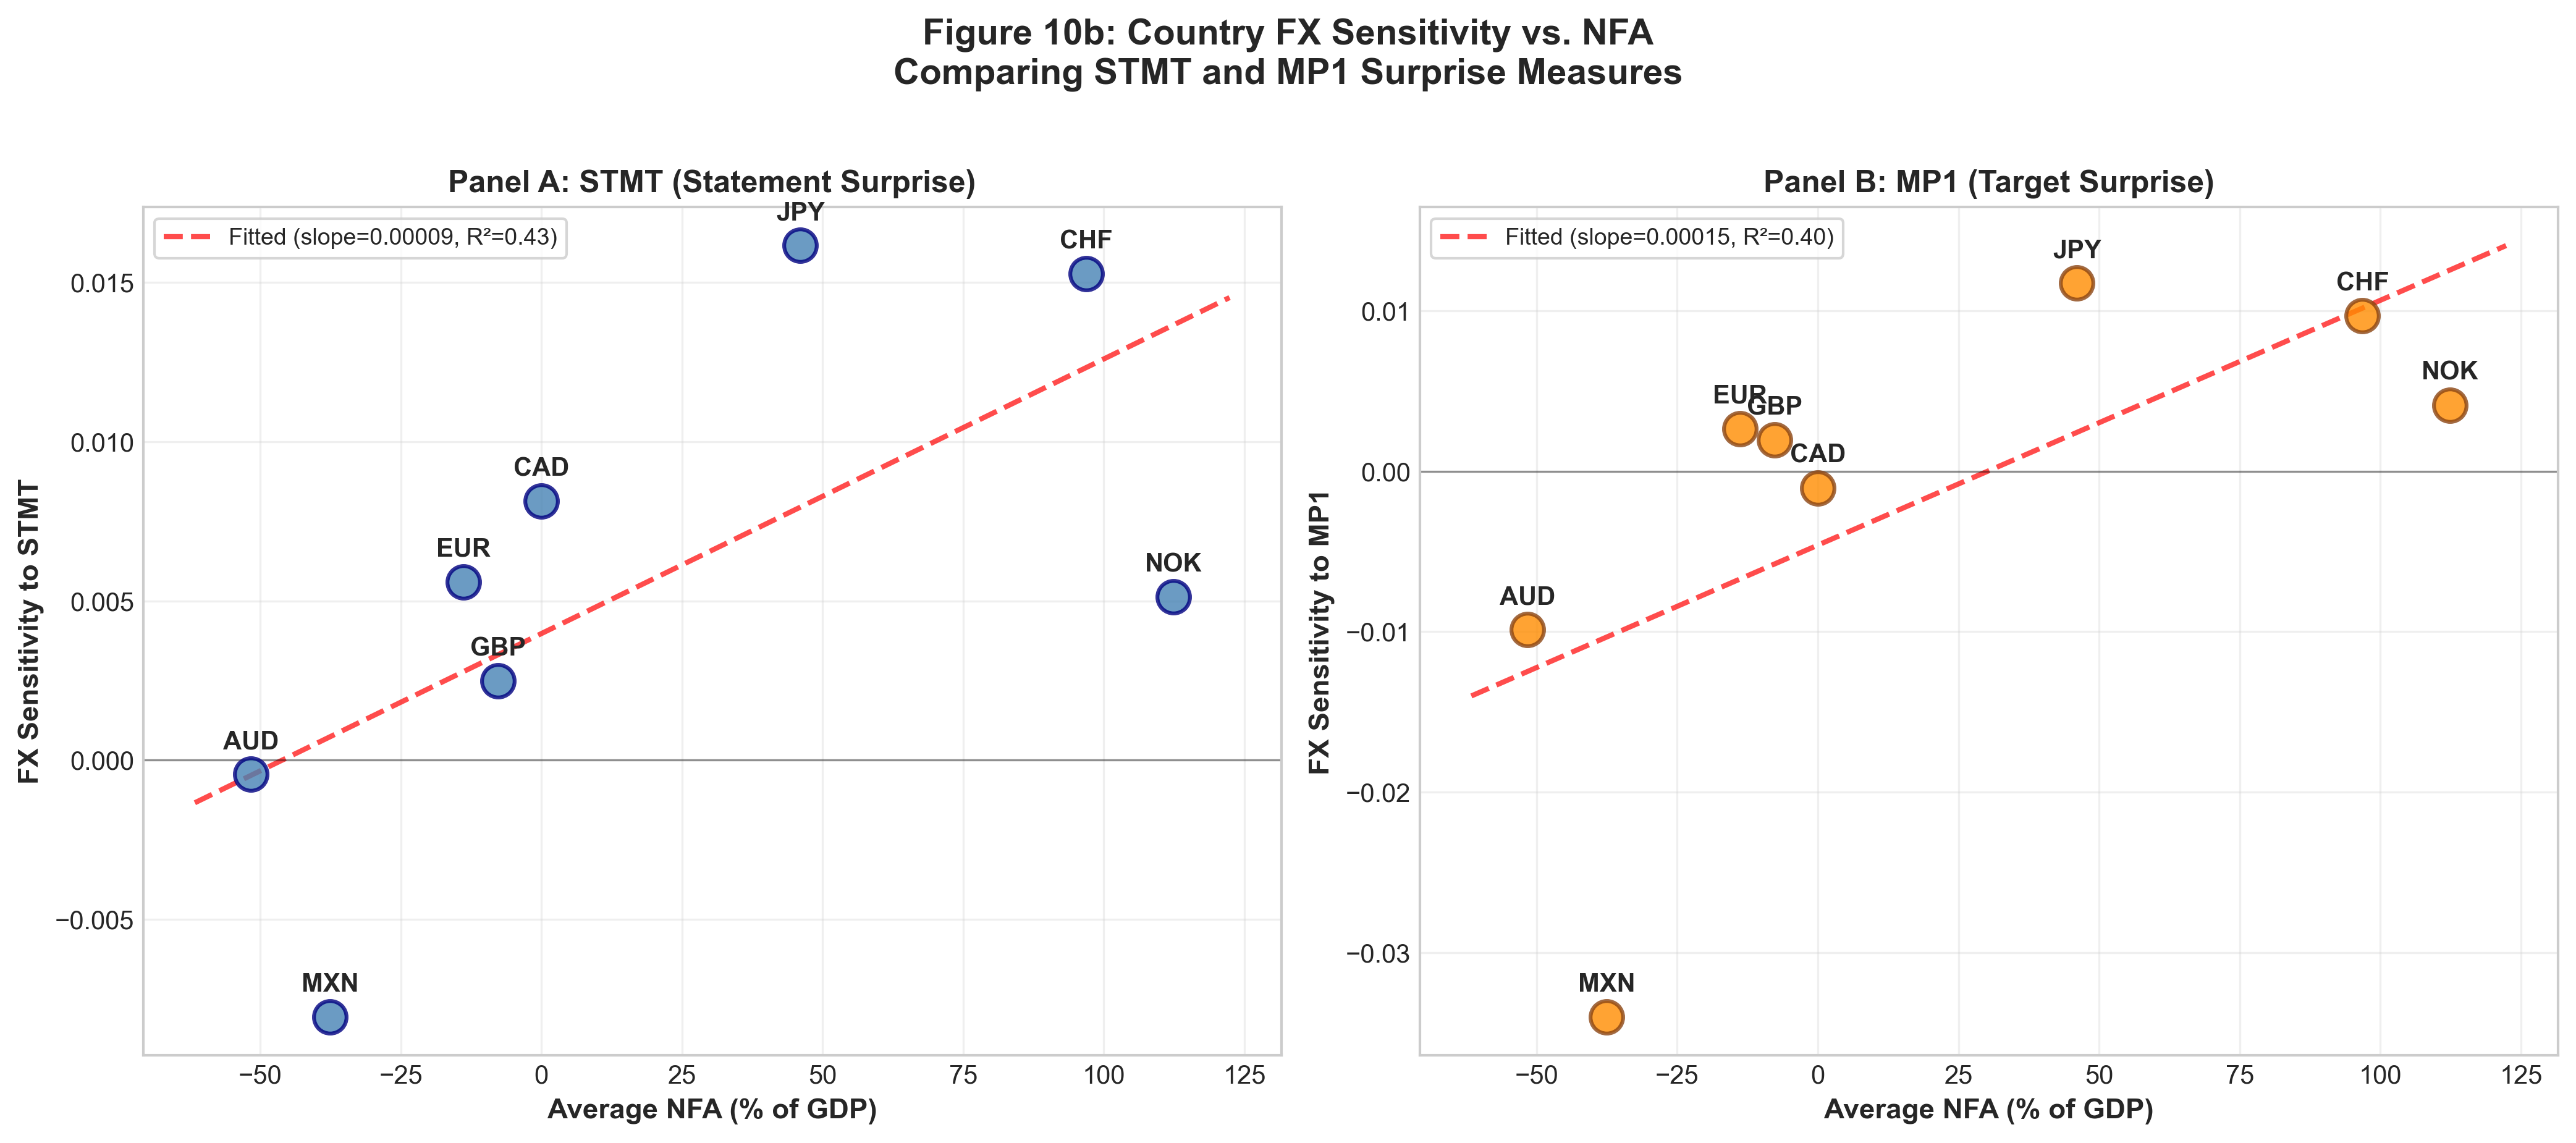
\includegraphics[width=\textwidth]{figure10b_betas_vs_nfa_both.png}
\caption{Country-specific FX betas vs.\ NFA/GDP: STMT and MP1 comparison.}
\end{figure}

\clearpage
% ----------------------------------------------------------------------------
\section{Figure 11: Marginal Effects}
\begin{figure}[H]
\centering
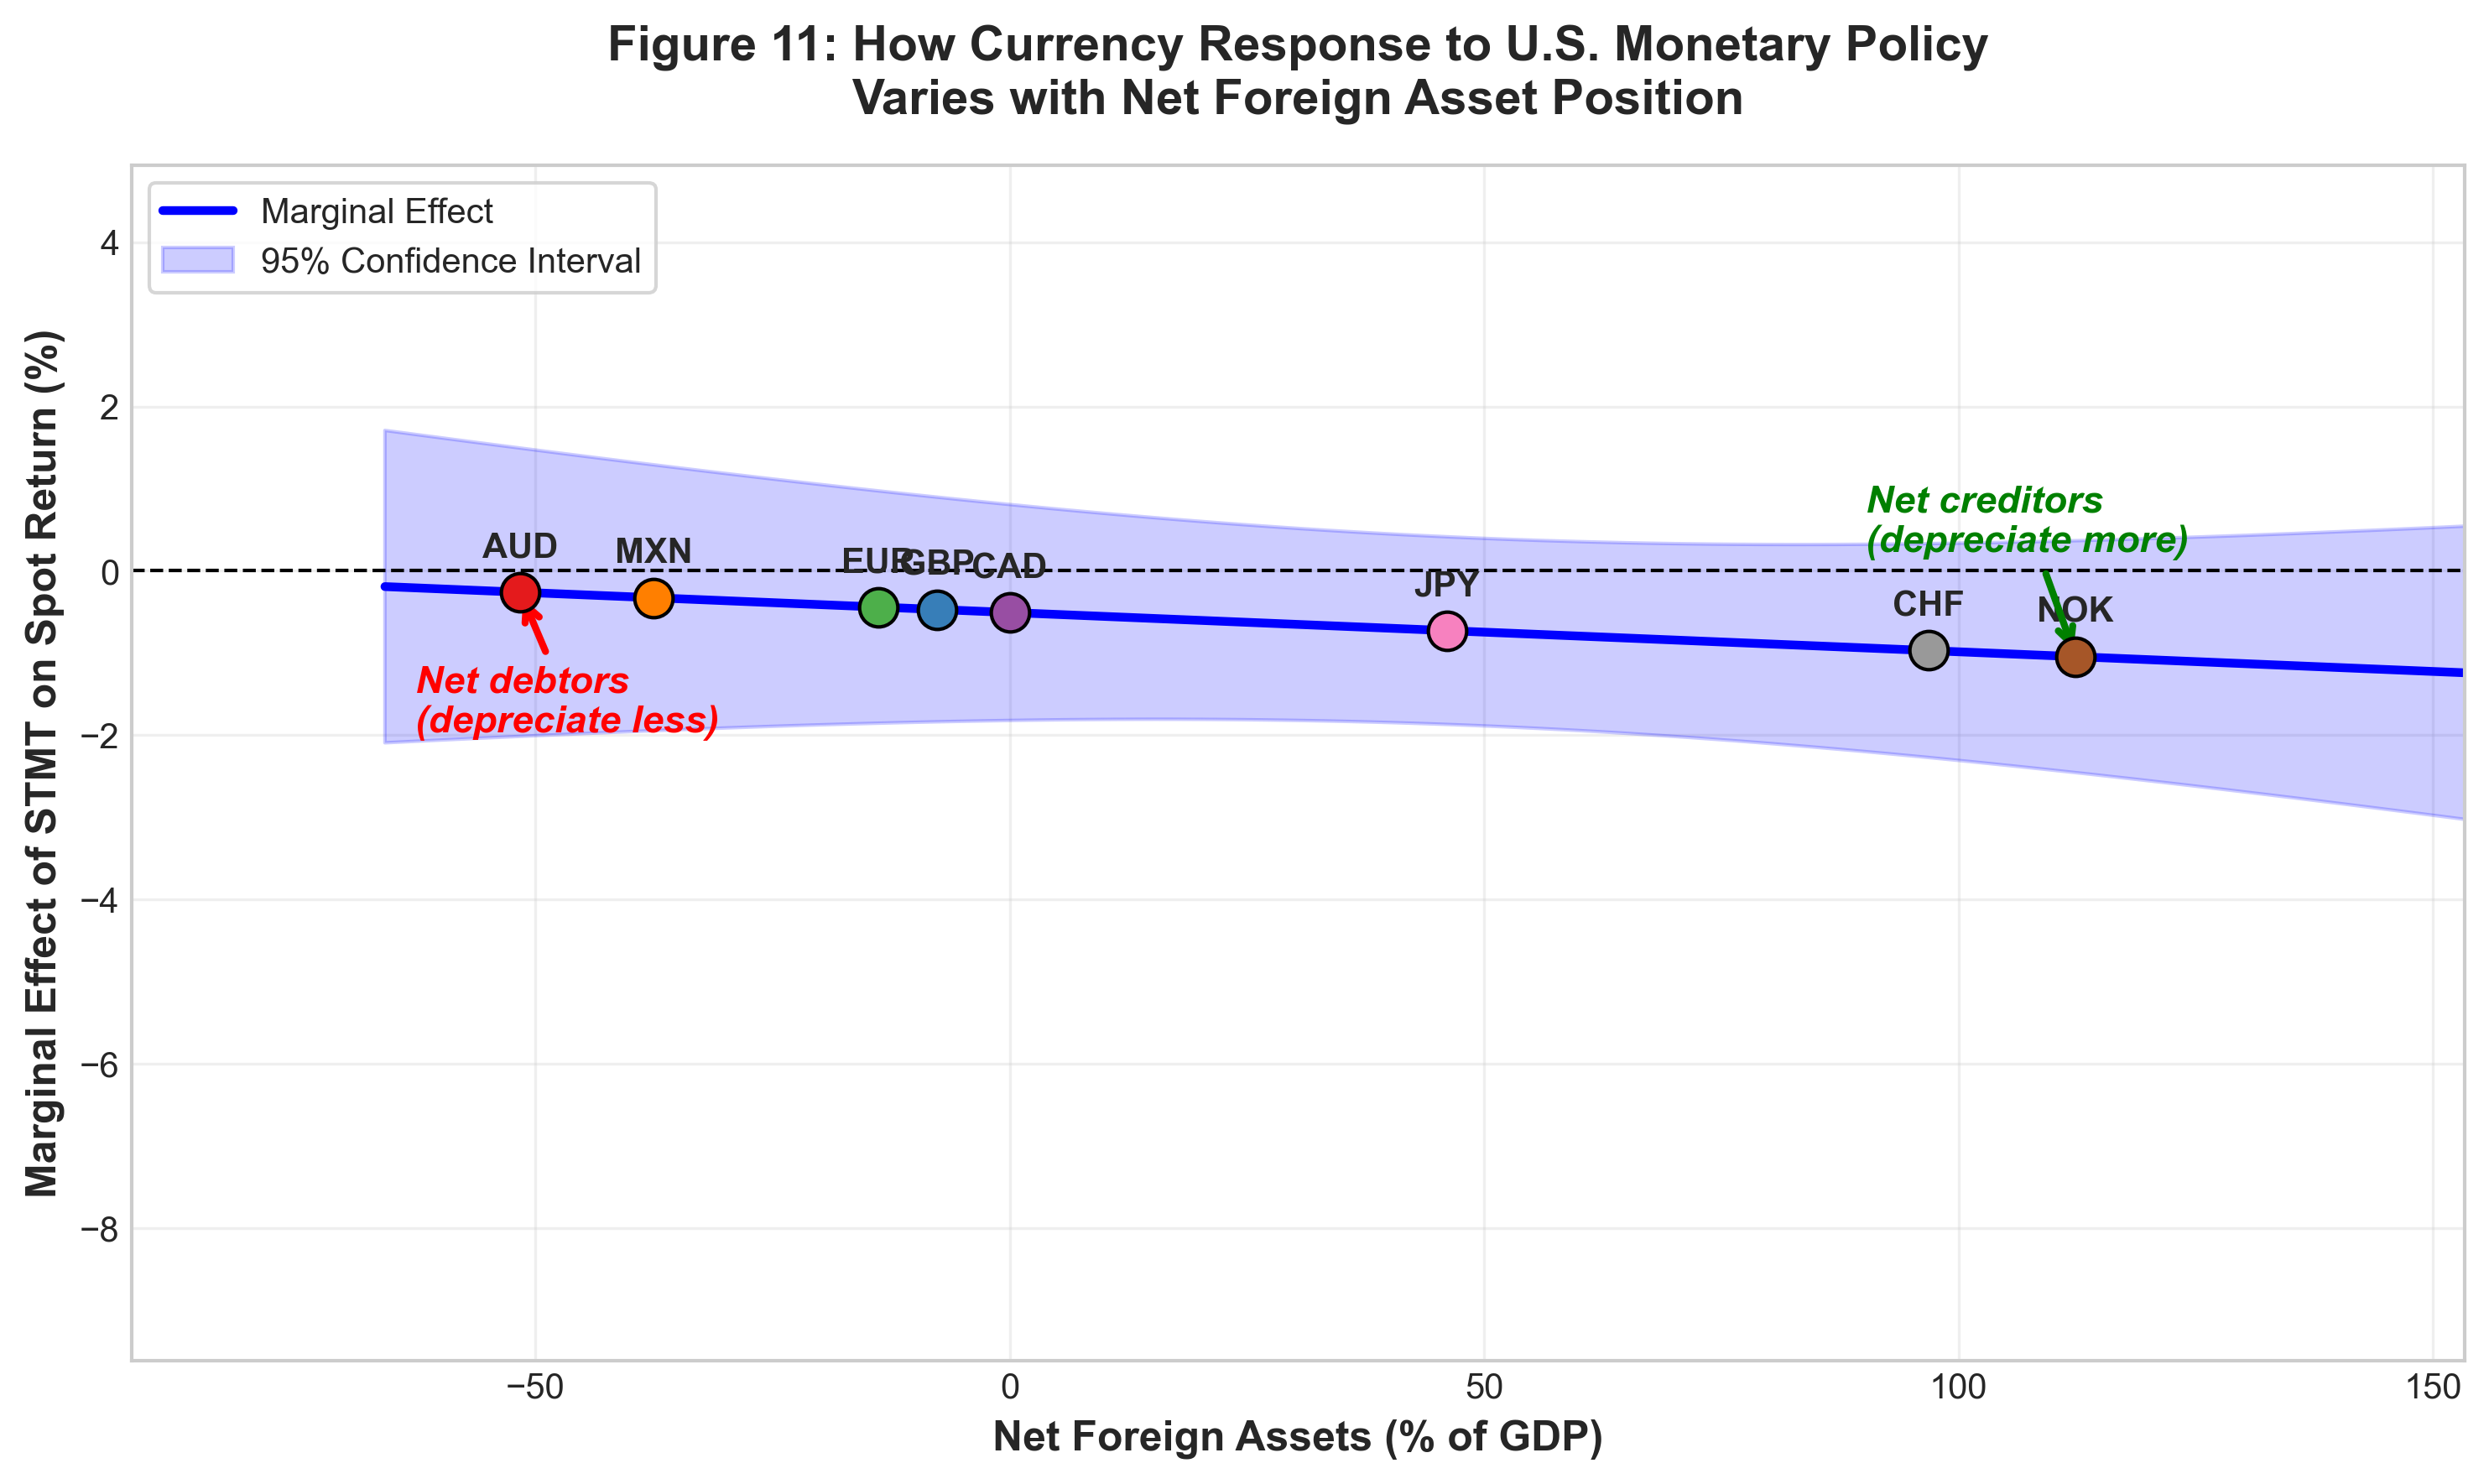
\includegraphics[width=\textwidth]{figure11_marginal_effects.png}
\caption{Marginal effects of monetary policy surprise conditional on NFA/GDP.}
\end{figure}

\clearpage
% ----------------------------------------------------------------------------
\section{Figure 12: Predicted Responses}
\begin{figure}[H]
\centering
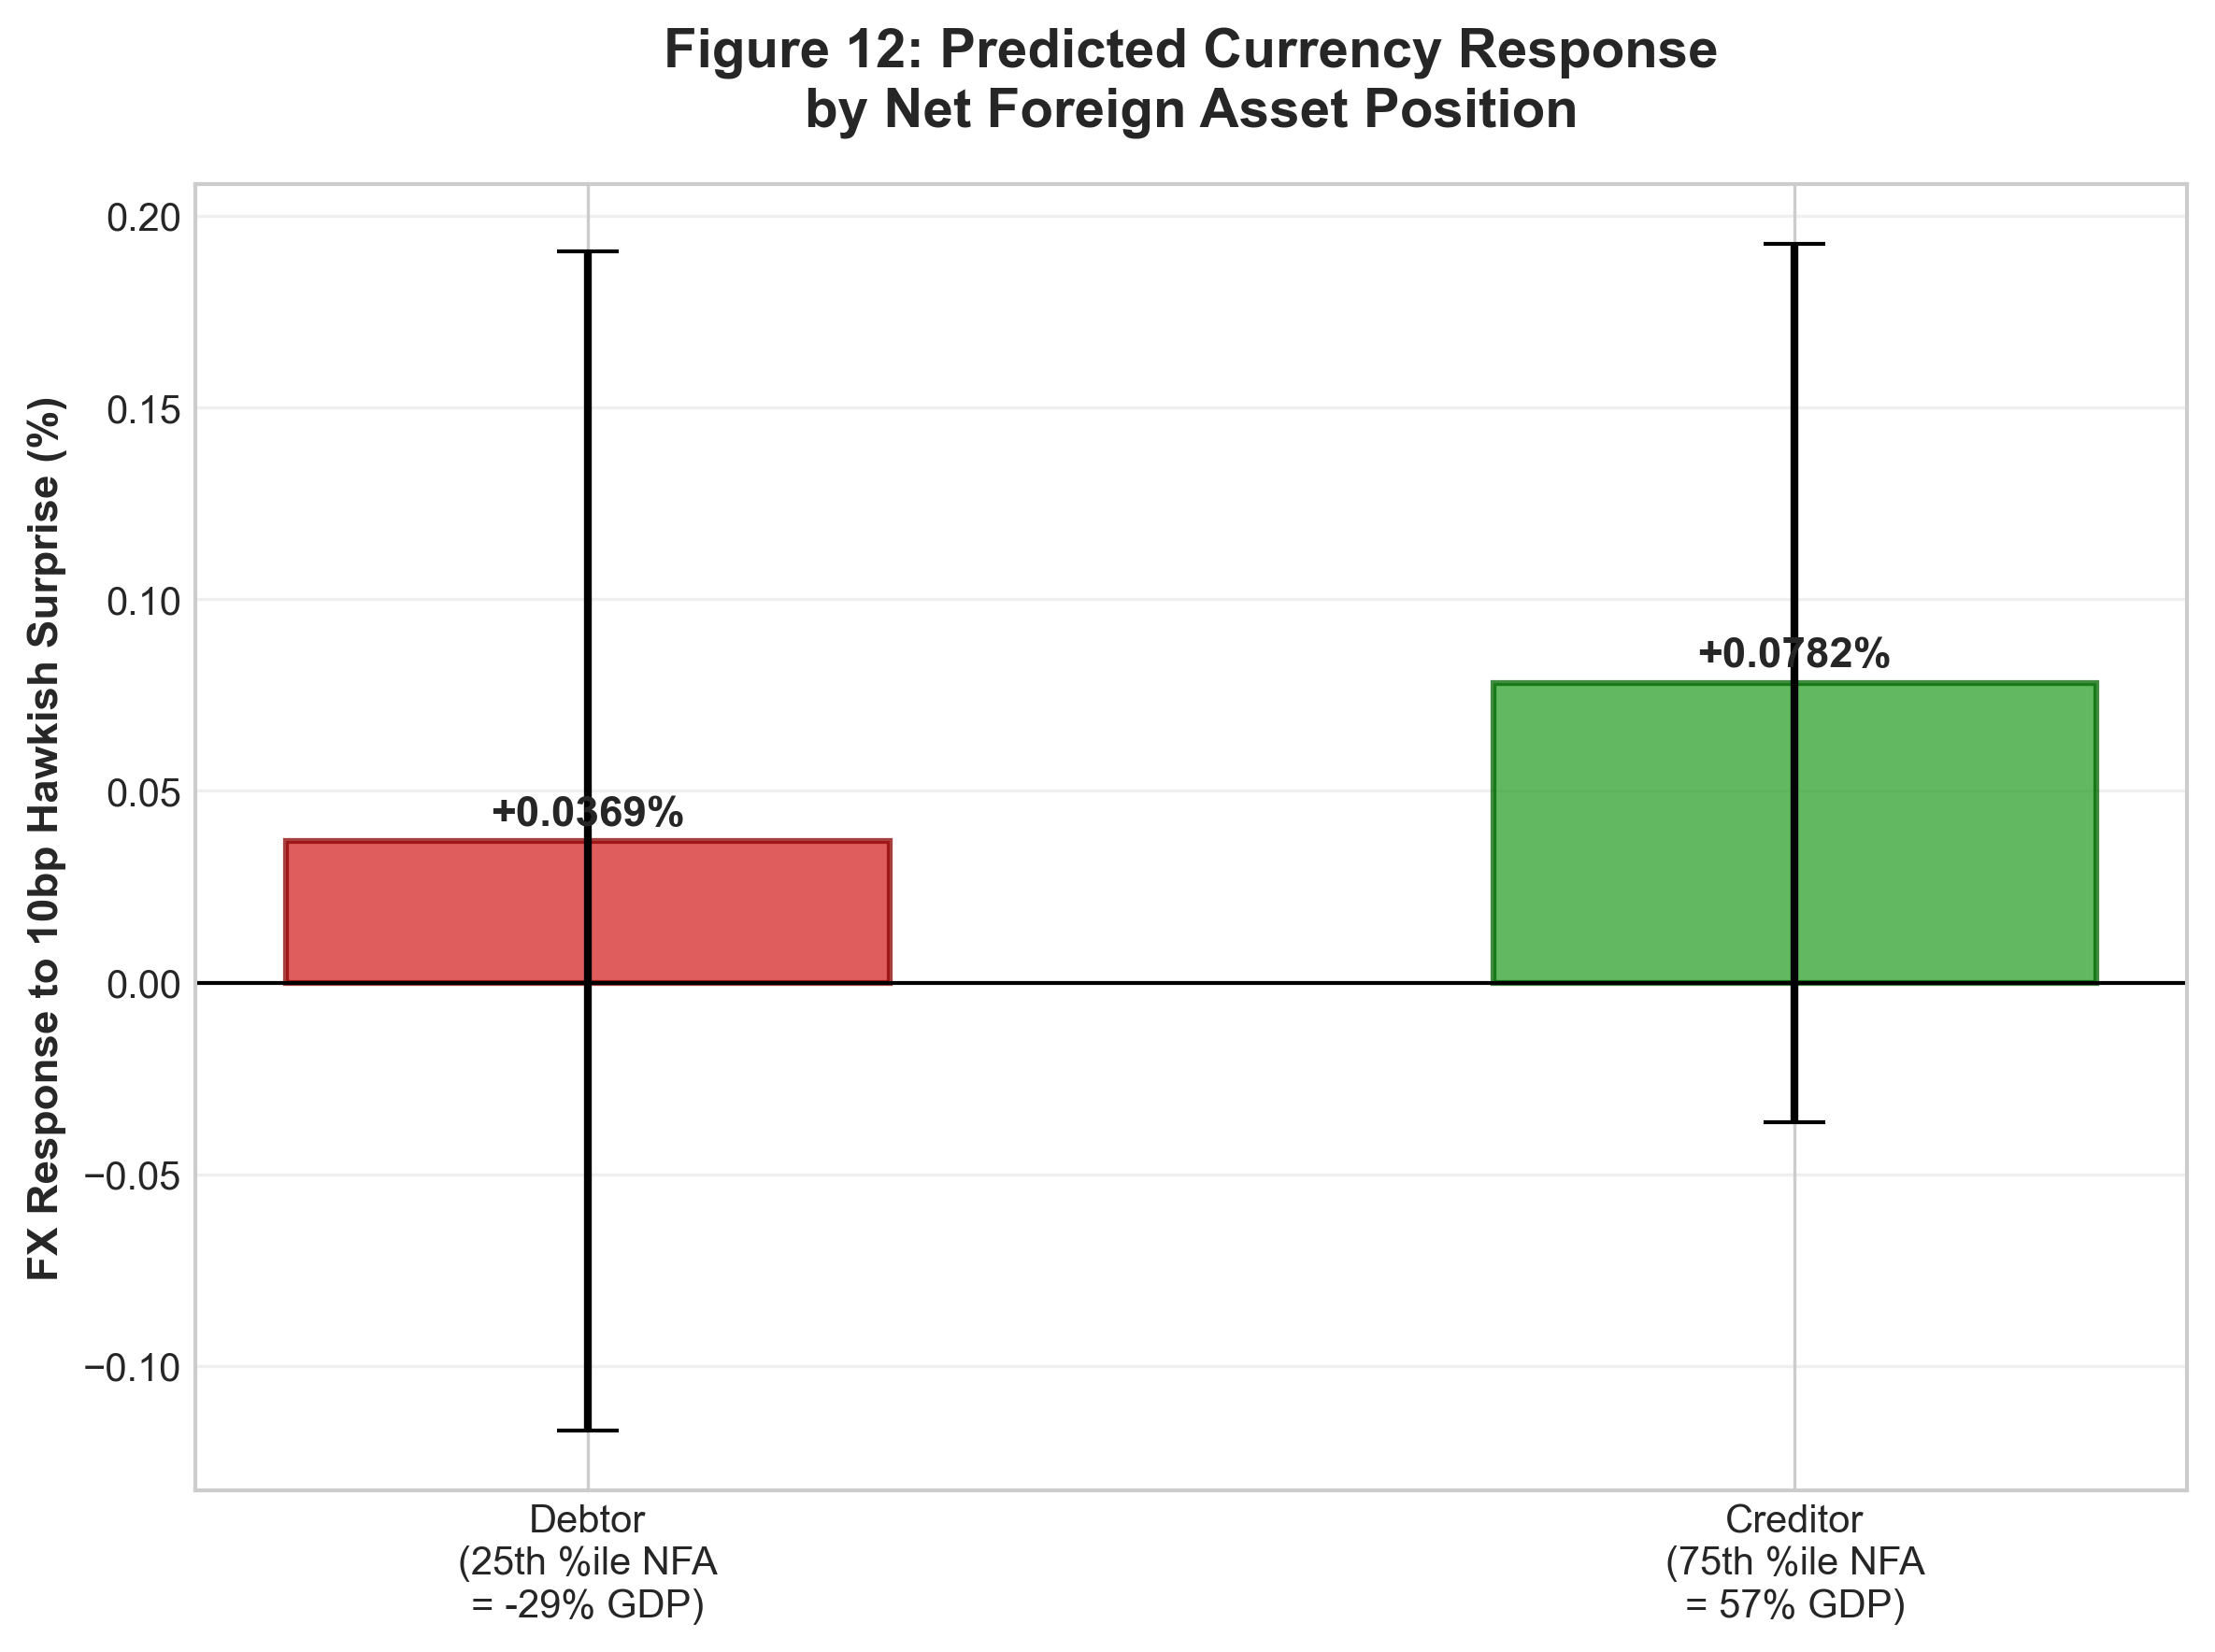
\includegraphics[width=\textwidth]{figure12_predicted_responses.png}
\caption{Model-predicted FX responses by NFA quintile.}
\end{figure}

\clearpage
% ----------------------------------------------------------------------------
\section{Figure 13: Time Variation}
\begin{figure}[H]
\centering
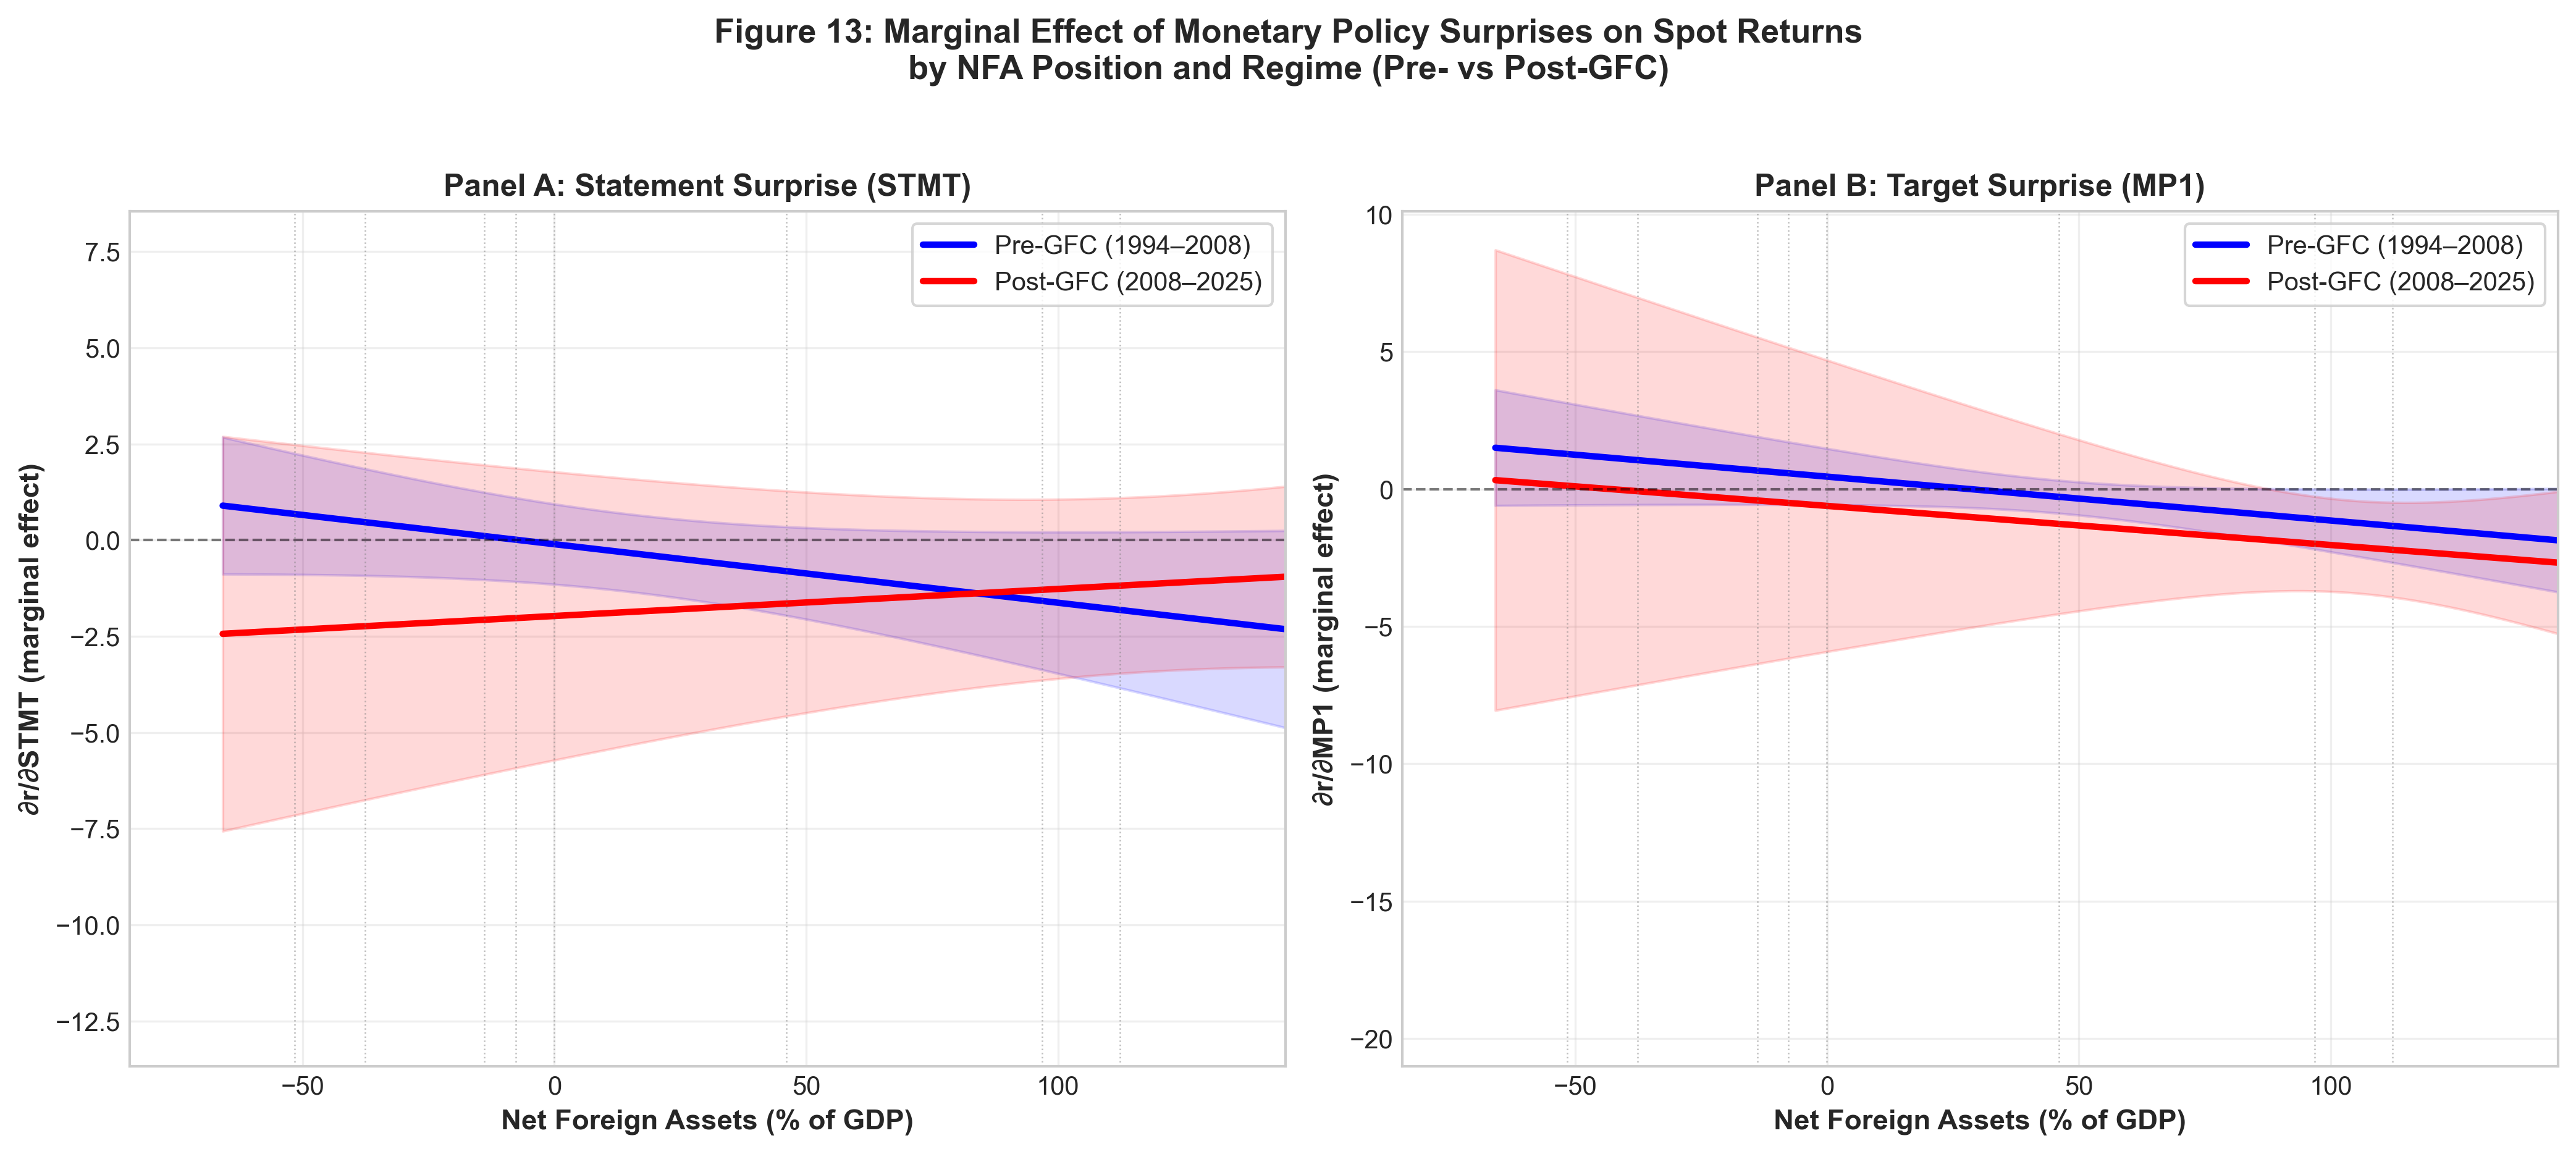
\includegraphics[width=\textwidth]{figure13_time_variation.png}
\caption{Time variation in NFA channel: pre-GFC vs.\ post-GFC comparison.}
\end{figure}

\clearpage
% ----------------------------------------------------------------------------
\section{Figure 14: Coefficient Comparison}
\begin{figure}[H]
\centering
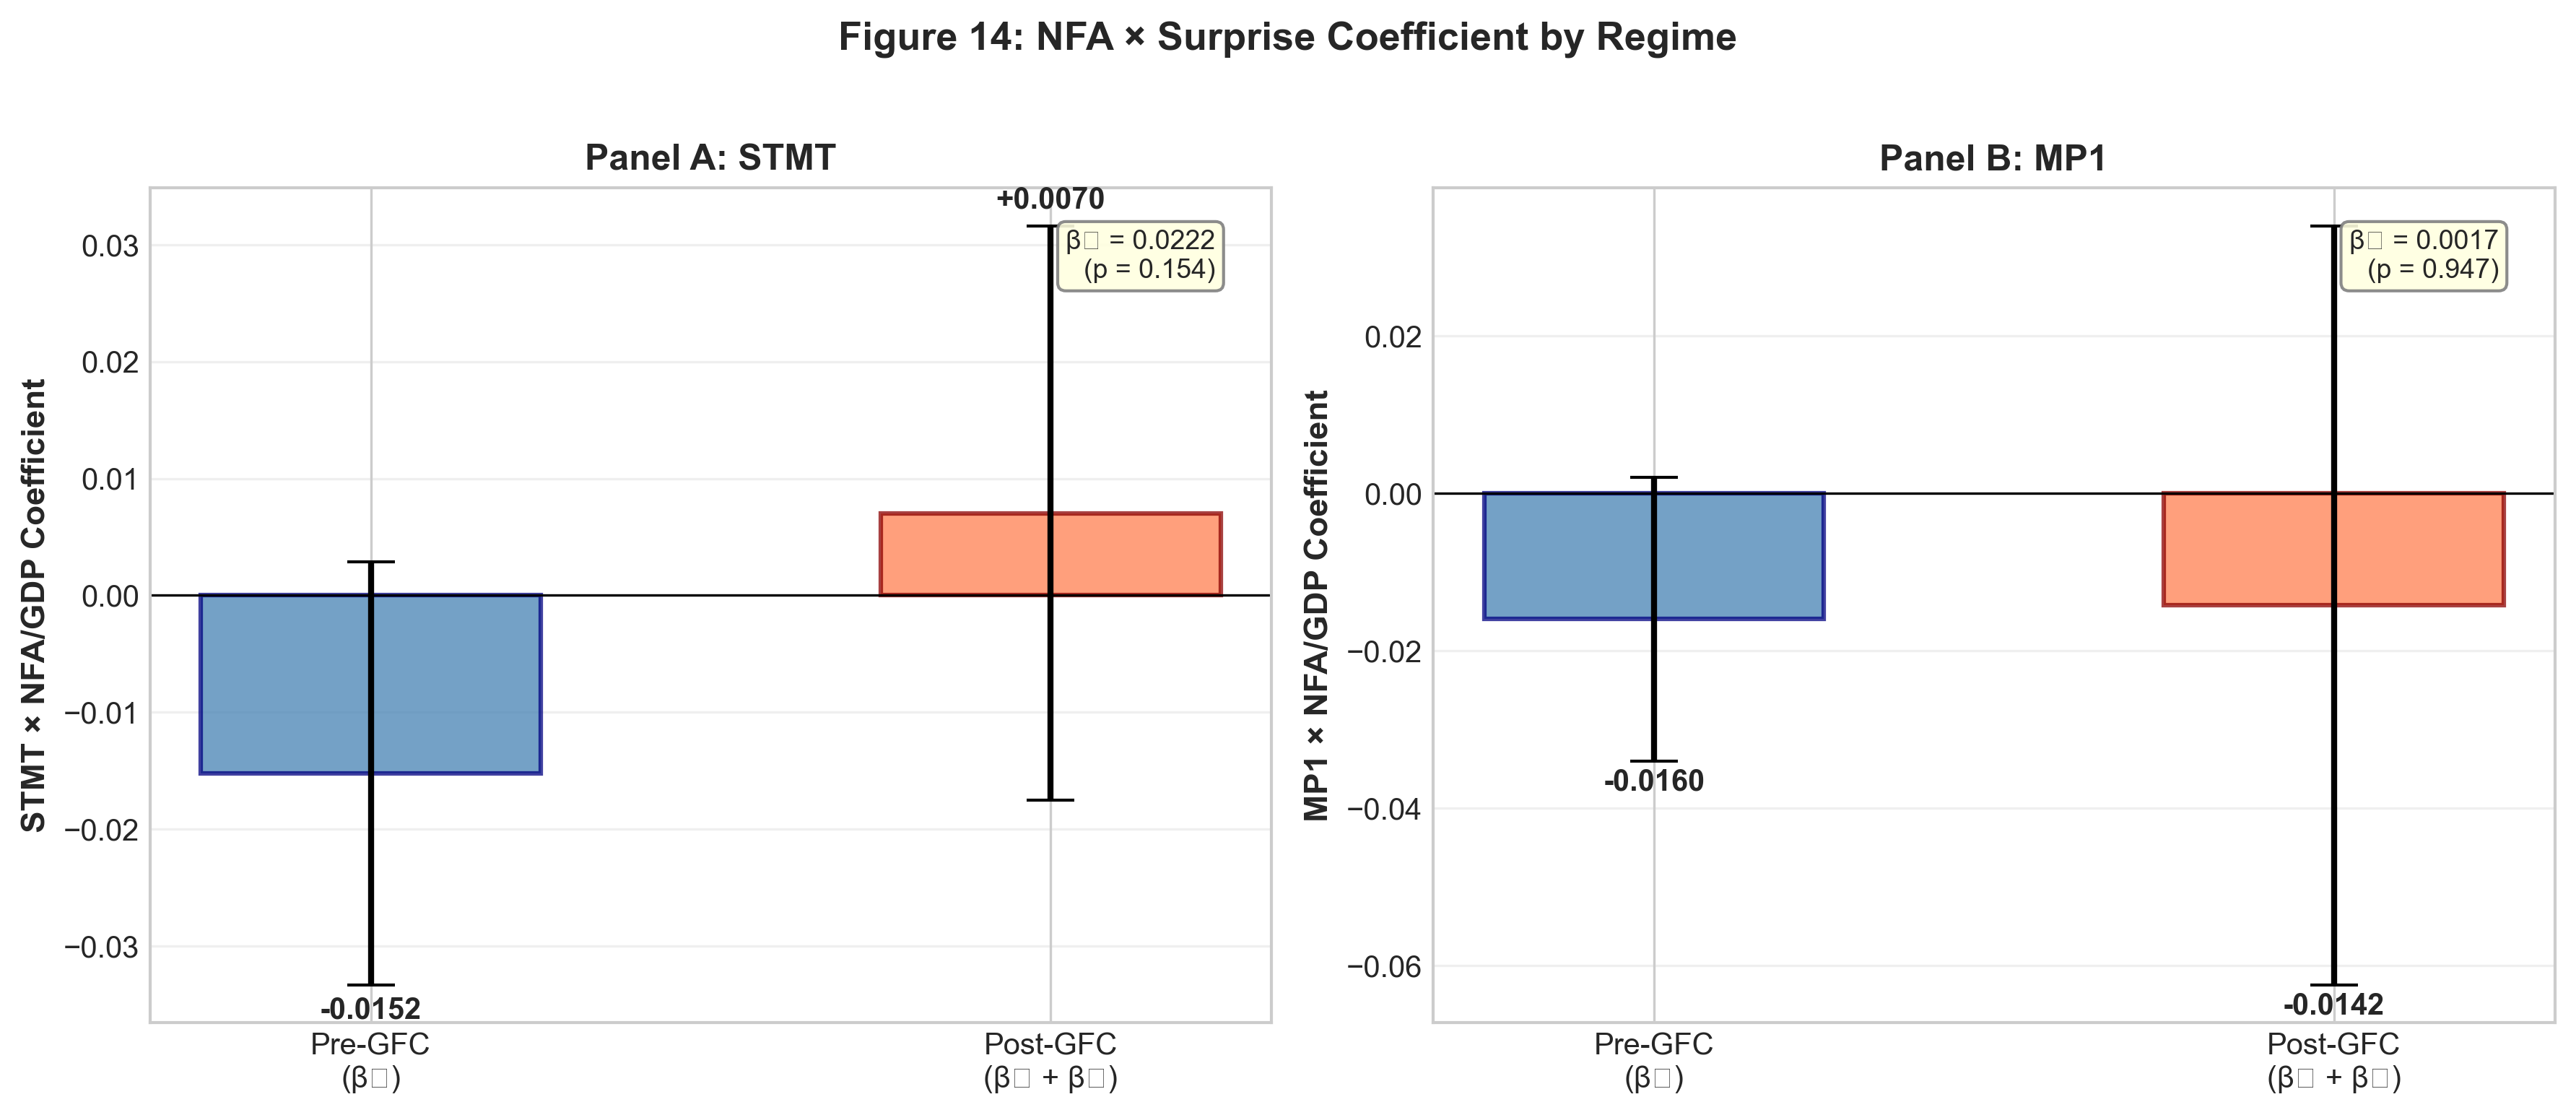
\includegraphics[width=\textwidth]{figure14_coefficient_comparison.png}
\caption{Coefficient comparison across model specifications.}
\end{figure}

\clearpage
% ----------------------------------------------------------------------------
\section{Figure 15: VIX Stress}
\begin{figure}[H]
\centering
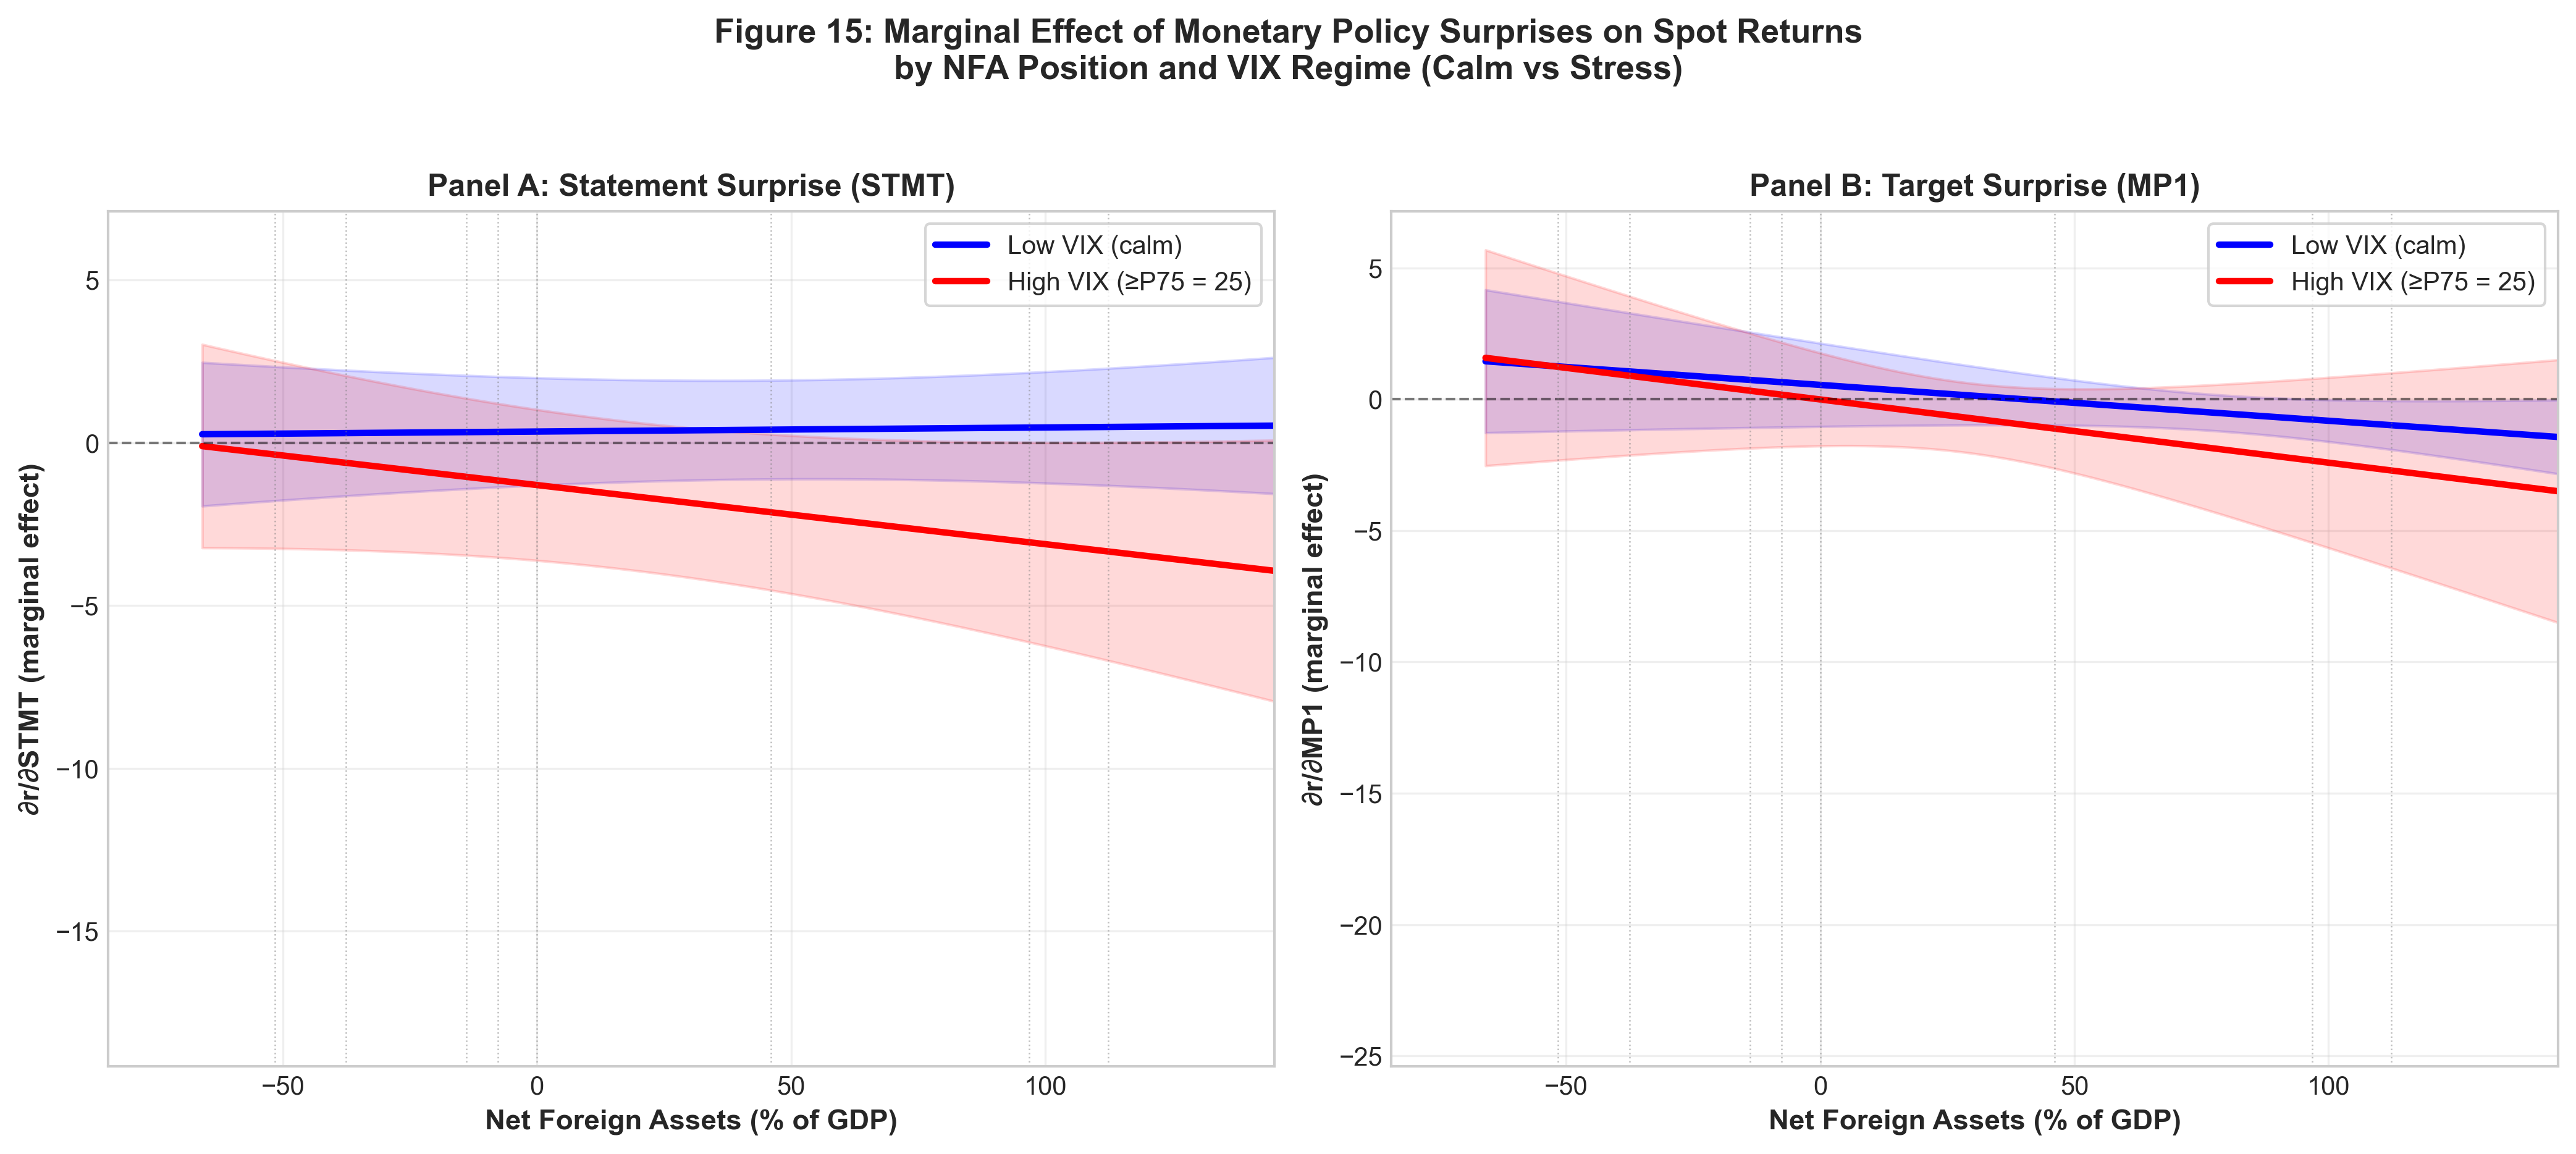
\includegraphics[width=\textwidth]{figure15_vix_stress.png}
\caption{NFA channel during high-VIX stress episodes.}
\end{figure}

\clearpage
% ----------------------------------------------------------------------------
\section{Figure 16: VIX Coefficient Comparison}
\begin{figure}[H]
\centering
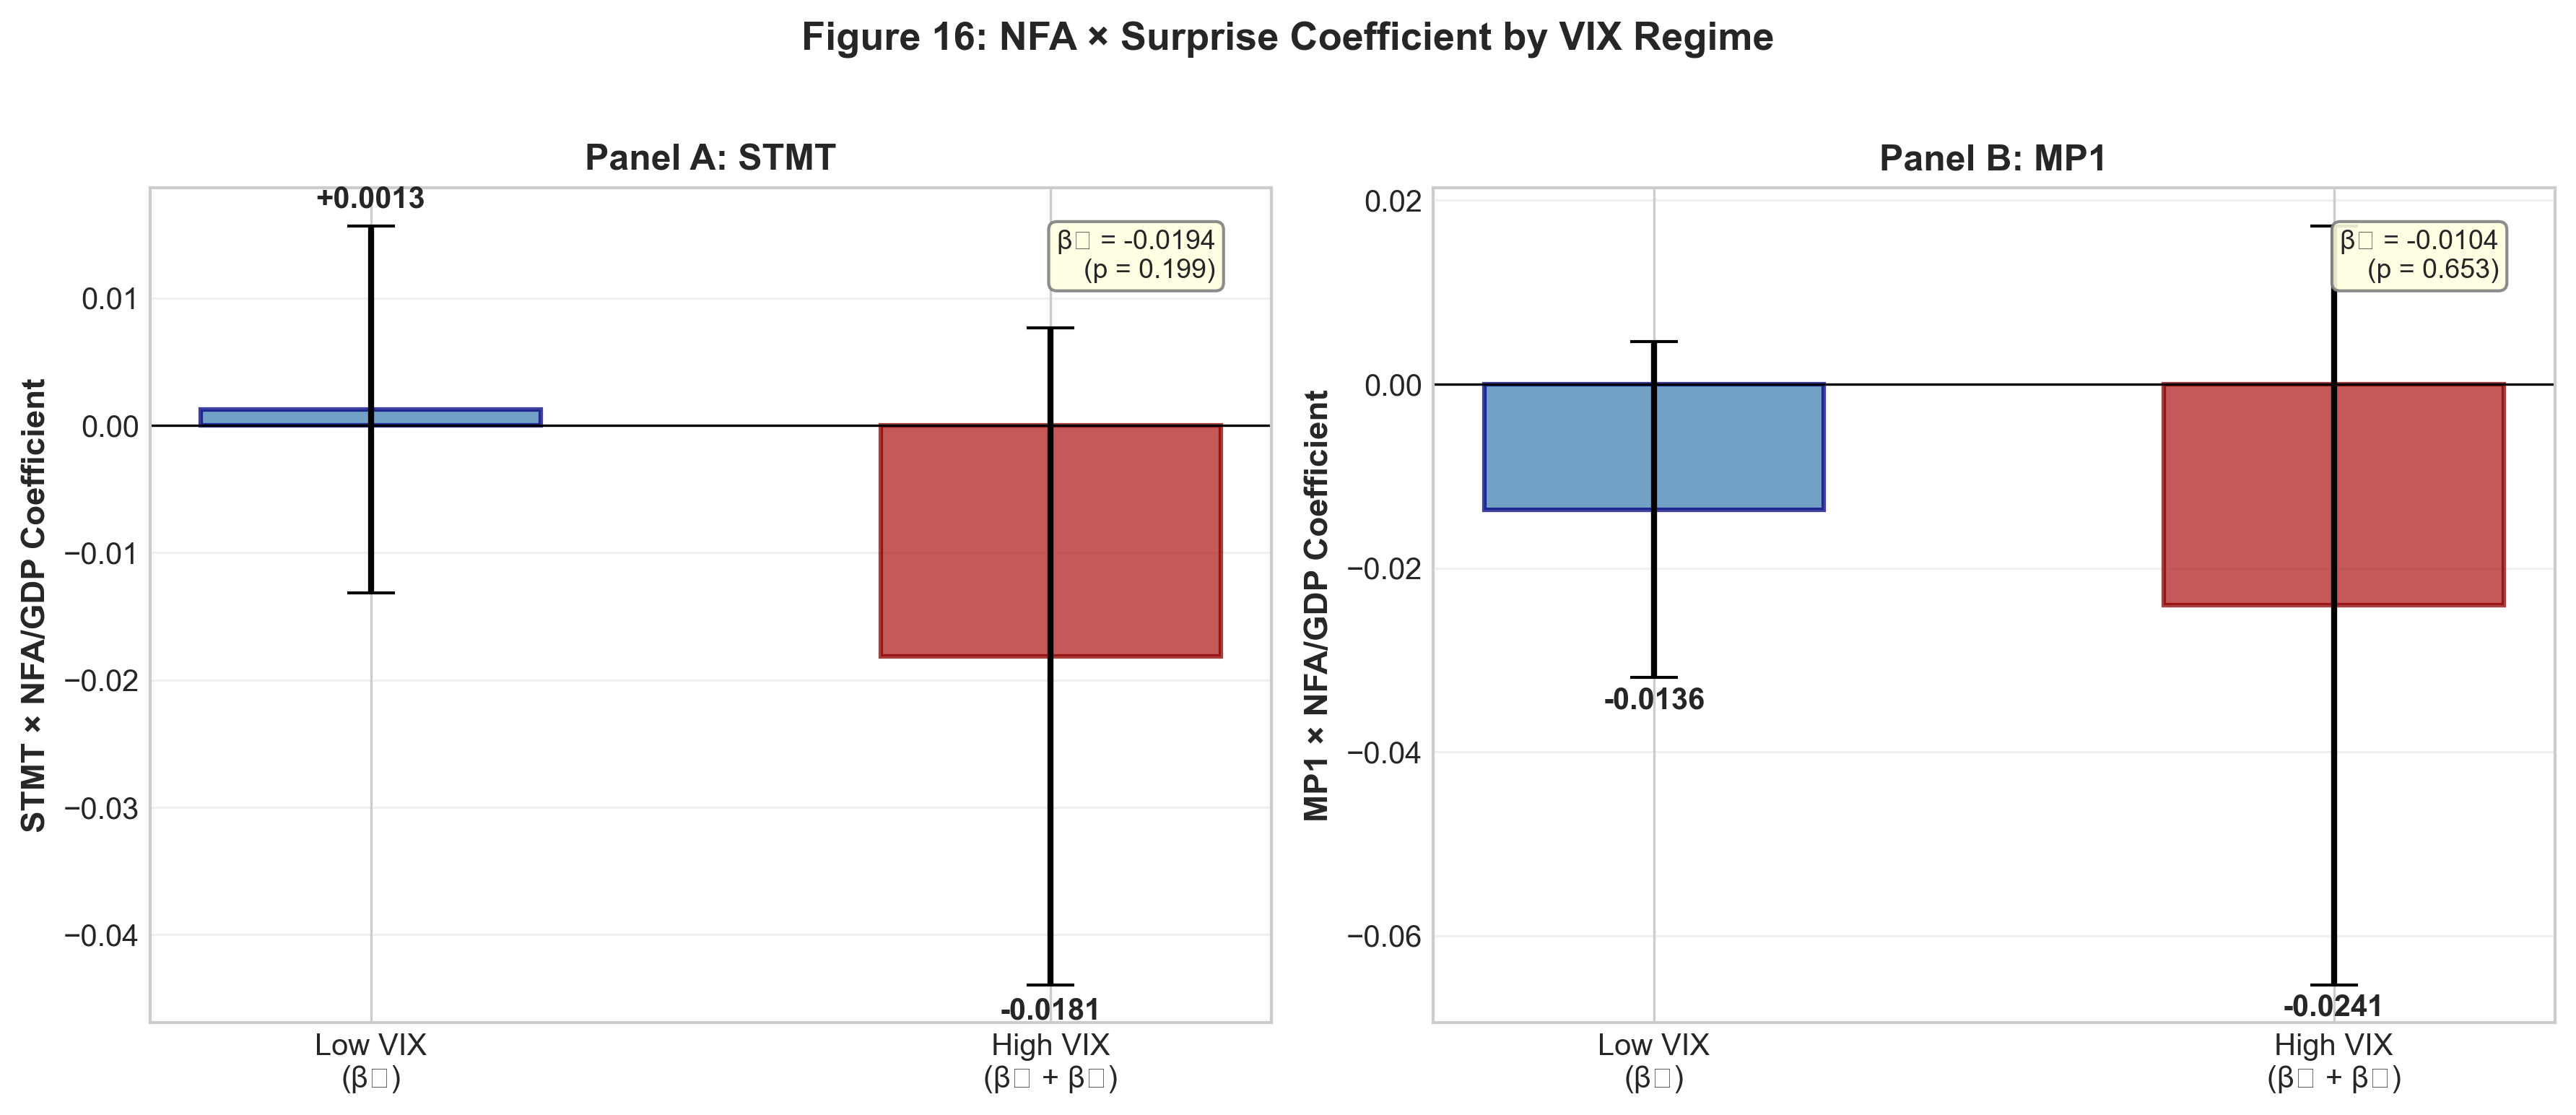
\includegraphics[width=\textwidth]{figure16_vix_coefficient_comparison.png}
\caption{Coefficient comparison: normal vs.\ high-VIX regimes.}
\end{figure}

\clearpage

% ============================================================================
% PART III: SUPPLEMENTARY MATERIALS
% ============================================================================
\part{Supplementary Materials}
\clearpage

\section{Writeup}
The complete analysis writeup is provided as a separate document:

\begin{itemize}
    \item \textbf{writeup.pdf} --- Main submission ($\sim$5 pages text + tables/figures)
\end{itemize}

\section{Code Repository}
All source code is available at:
\url{https://github.com/Toba4366/MIT-Coding-Challenge}

\section{AI Assistance}
\textit{\small AI assistance was used in this project. Conversation logs are available at \url{https://chatgpt.com/share/69980c6a-51cc-8012-b12c-9eac1e7f4b44} and in the References/AI folder.}

\end{document}
